%!TEX TS-program = xelatex
\documentclass[notes,12pt, aspectratio=169]{beamer}

\usepackage{amsmath,amsfonts,amssymb,amsthm,mathtools}  % пакеты для математики
\usepackage{minted}

\usepackage[english, russian]{babel} % выбор языка для документа
\usepackage[utf8]{inputenc} % задание utf8 кодировки исходного tex файла
\usepackage[X2,T2A]{fontenc}        % кодировка

\usepackage{fontspec}         % пакет для подгрузки шрифтов
\setmainfont{Helvetica}  % задаёт основной шрифт документа

% why do we need \newfontfamily:
% http://tex.stackexchange.com/questions/91507/
\newfontfamily{\cyrillicfonttt}{Helvetica}
\newfontfamily{\cyrillicfont}{Helvetica}
\newfontfamily{\cyrillicfontsf}{Helvetica}

\usepackage{unicode-math}     % пакет для установки математического шрифта
% \setmathfont{Neo Euler} % шрифт для математики

\usepackage{polyglossia}      % Пакет, который позволяет подгружать русские буквы
\setdefaultlanguage{russian}  % Основной язык документа
\setotherlanguage{english}    % Второстепенный язык документа

% Шрифт для кода
\setmonofont[Scale=0.85]{Monaco}
\usepackage{verbments}

\usepackage{pgfpages}
% These slides also contain speaker notes. You can print just the slides,
% just the notes, or both, depending on the setting below. Comment out the want
% you want.
%\setbeameroption{hide notes} % Only slide
%\setbeameroption{show only notes} % Only notes
%\setbeameroption{show notes on second screen=right} % Both

\usepackage{array}

\usepackage{tikz}
\usepackage{verbatim}
\setbeamertemplate{note page}{\pagecolor{yellow!5}\insertnote}
\usetikzlibrary{positioning}
\usetikzlibrary{snakes}
\usetikzlibrary{calc}
\usetikzlibrary{arrows}
\usetikzlibrary{decorations.markings}
\usetikzlibrary{shapes.misc}
\usetikzlibrary{matrix,shapes,arrows,fit,tikzmark}

\usepackage{hyperref}
\usepackage{lipsum}
\usepackage{multimedia}
\usepackage{multirow}
\usepackage{dcolumn}
\usepackage{bbm}
\newcolumntype{d}[0]{D{.}{.}{5}}

\usepackage{changepage}
\usepackage{appendixnumberbeamer}
\newcommand{\beginbackup}{
   \newcounter{framenumbervorappendix}
   \setcounter{framenumbervorappendix}{\value{framenumber}}
   \setbeamertemplate{footline}
   {
     \leavevmode%
     \hline
     box{%
       \begin{beamercolorbox}[wd=\paperwidth,ht=2.25ex,dp=1ex,right]{footlinecolor}%
%         \insertframenumber  \hspace*{2ex} 
       \end{beamercolorbox}}%
     \vskip0pt%
   }
 }
\newcommand{\backupend}{
   \addtocounter{framenumbervorappendix}{-\value{framenumber}}
   \addtocounter{framenumber}{\value{framenumbervorappendix}} 
}

% для имитации питоновского синтаксиса 
\newcommand{\pgr}[1]{{\color{green} \textbf{#1}}}


%%%%%%%%%% Работа с картинками %%%%%%%%%
\usepackage{graphicx}                  % Для вставки рисунков
\usepackage{graphics}
\graphicspath{{images_4/}}    % можно указать папки с картинками
\usepackage{wrapfig}                   % Обтекание рисунков и таблиц текстом

\usepackage[space]{grffile}
\usepackage{booktabs}

% These are my colors -- there are many like them, but these ones are mine.
\definecolor{blue}{RGB}{0,114,178}
\definecolor{red}{RGB}{213,94,0}
\definecolor{yellow}{RGB}{240,228,66}
\definecolor{green}{RGB}{0,128, 0}

\hypersetup{
  colorlinks=false,
  linkbordercolor = {white},
  linkcolor = {blue}
}


%% I use a beige off white for my background
\definecolor{MyBackground}{RGB}{255,253,218}

%% Uncomment this if you want to change the background color to something else
%\setbeamercolor{background canvas}{bg=MyBackground}

%% Change the bg color to adjust your transition slide background color!
\newenvironment{transitionframe}{
  \setbeamercolor{background canvas}{bg=yellow}
  \begin{frame}}{
    \end{frame}
}

\setbeamercolor{frametitle}{fg=blue}
\setbeamercolor{title}{fg=black}
\setbeamertemplate{footline}[frame number]
\setbeamertemplate{navigation symbols}{} 
\setbeamertemplate{itemize items}{-}
\setbeamercolor{itemize item}{fg=blue}
\setbeamercolor{itemize subitem}{fg=blue}
\setbeamercolor{enumerate item}{fg=blue}
\setbeamercolor{enumerate subitem}{fg=blue}
\setbeamercolor{button}{bg=MyBackground,fg=blue,}


% If you like road maps, rather than having clutter at the top, have a roadmap show up at the end of each section 
% (and after your introduction)
% Uncomment this is if you want the roadmap!
% \AtBeginSection[]
% {
%    \begin{frame}
%        \frametitle{Roadmap of Talk}
%        \tableofcontents[currentsection]
%    \end{frame}
% }
\setbeamercolor{section in toc}{fg=blue}
\setbeamercolor{subsection in toc}{fg=red}
\setbeamersize{text margin left=1em,text margin right=1em} 

% списки, которые растягиваются на всю величину слайда 
\newenvironment{wideitemize}{\itemize\addtolength{\itemsep}{10pt}}{\enditemize}



\title[]{\textcolor{blue}{Практический анализ данных и машинное обучение: искусственные нейронные сети}}
\author{Ульянкин Филипп, Соловей Влад}
\date{\today}


\begin{document}

%%% TIKZ STUFF
\tikzset{   
        every picture/.style={remember picture,baseline},
        every node/.style={anchor=base,align=center,outer sep=1.5pt},
        every path/.style={thick},
        }
\newcommand\marktopleft[1]{%
    \tikz[overlay,remember picture] 
        \node (marker-#1-a) at (-.3em,.3em) {};%
}
\newcommand\markbottomright[2]{%
    \tikz[overlay,remember picture] 
        \node (marker-#1-b) at (0em,0em) {};%
}
\tikzstyle{every picture}+=[remember picture] 
\tikzstyle{mybox} =[draw=black, very thick, rectangle, inner sep=10pt, inner ysep=20pt]
\tikzstyle{fancytitle} =[draw=black,fill=red, text=white]
%%%% END TIKZ STUFF

% Title Slide
\begin{frame}
\maketitle
\centering Как научить компьютер читать, w2v
\end{frame}


\begin{frame}{Agenda} 
\begin{wideitemize}
	\item  Анализ текстов и логистическая регрессия 
	\item  Что такое embeddings, модель word2vec
	\item  Учим свой собственный w2v на википедии, сравниваем с чужим
	\item  Сентимент-анализ недавних событий по твиттеру
\end{wideitemize}
\end{frame}


\begin{transitionframe}
	\begin{center}
		\Huge  NLP (Natural Language Processing)
	\end{center}
\end{transitionframe}


{
	\usebackgroundtemplate{ 
		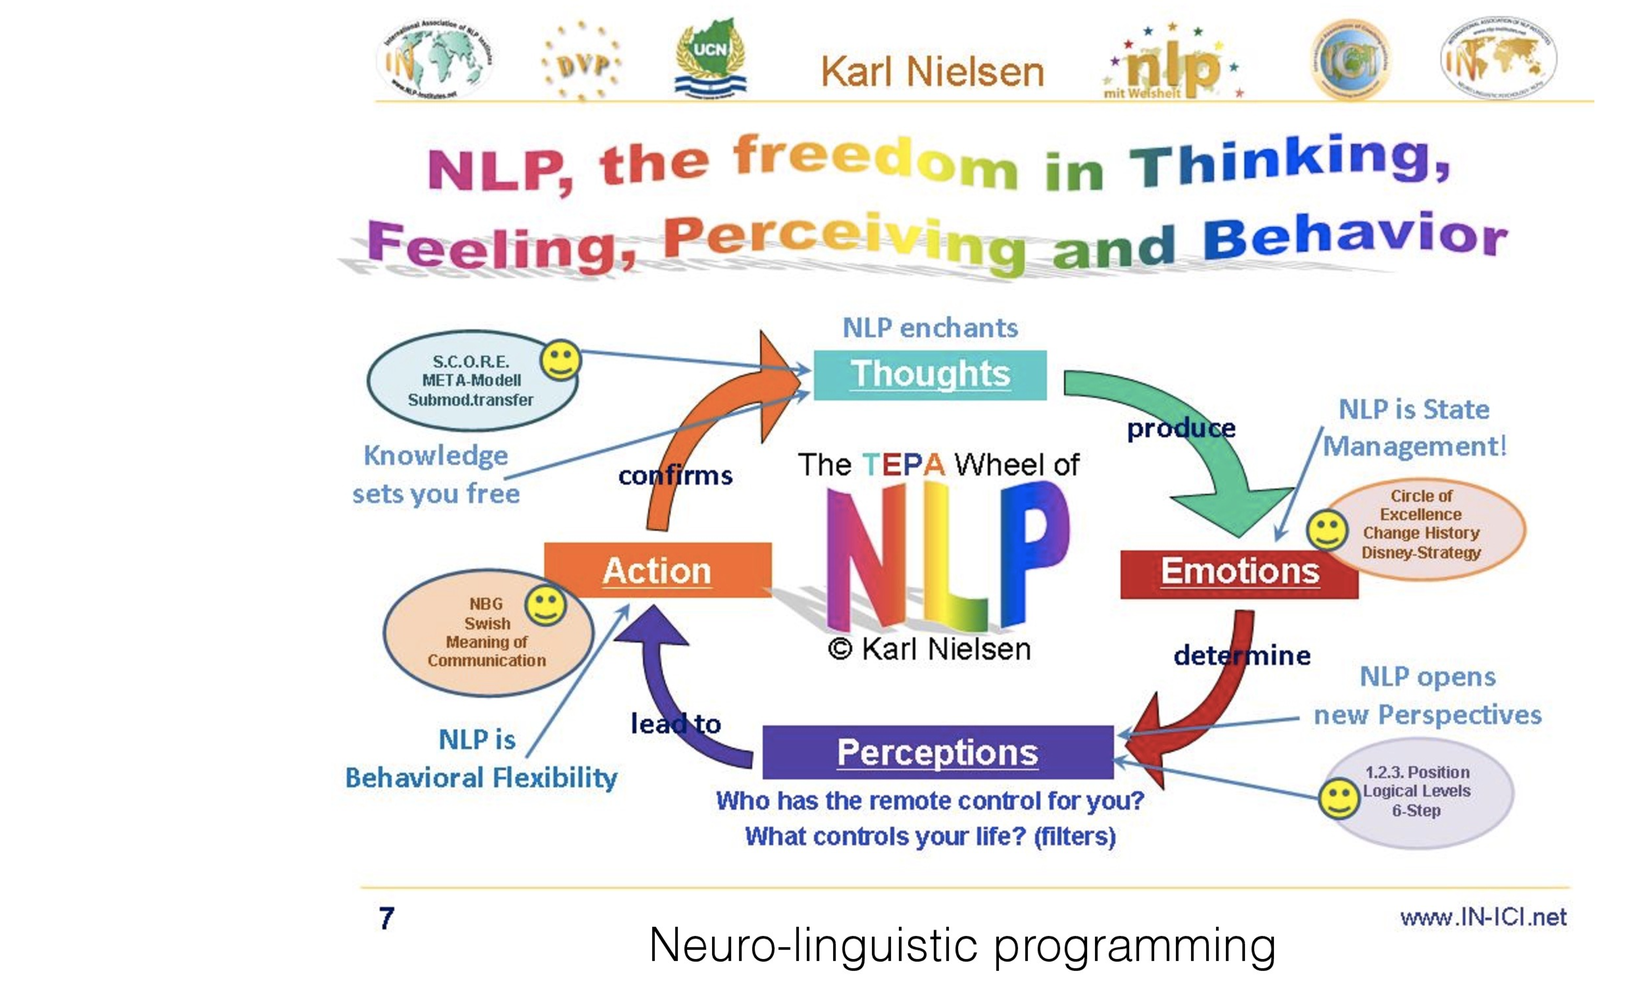
\includegraphics[width=0.83\paperwidth]{nlp1.png}}
	\begin{frame}
\end{frame}
}


{
	\usebackgroundtemplate{ 
		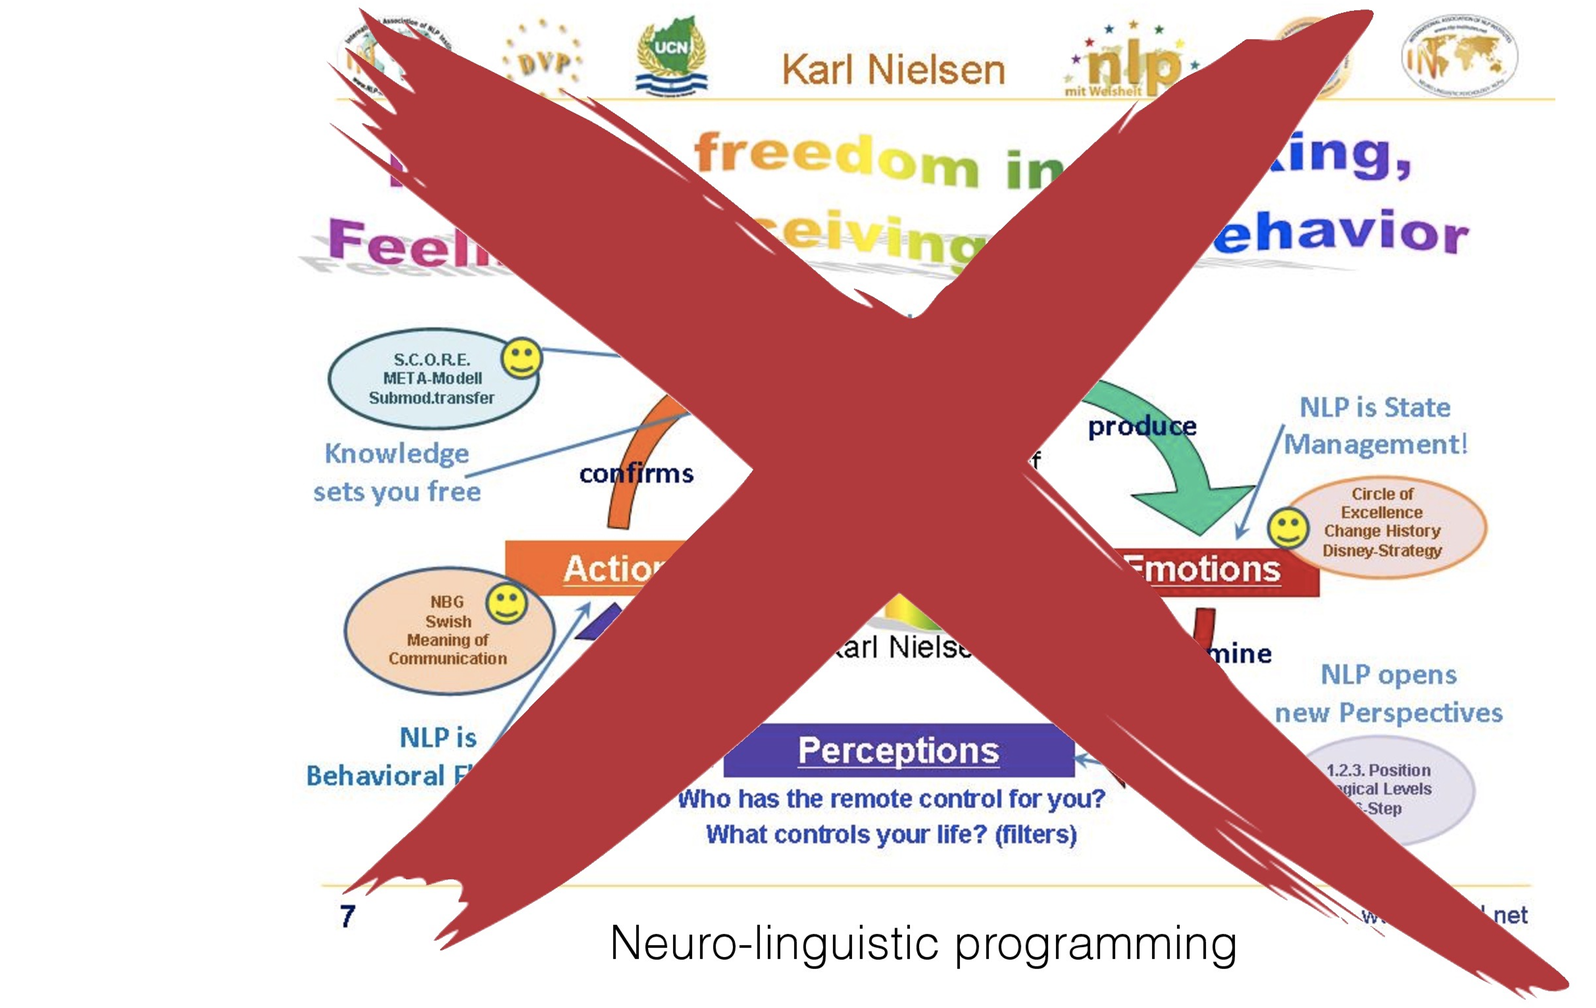
\includegraphics[width=0.83\paperwidth]{nlp2.png}}
	\begin{frame}
\end{frame}
}


{
	\usebackgroundtemplate{ 
		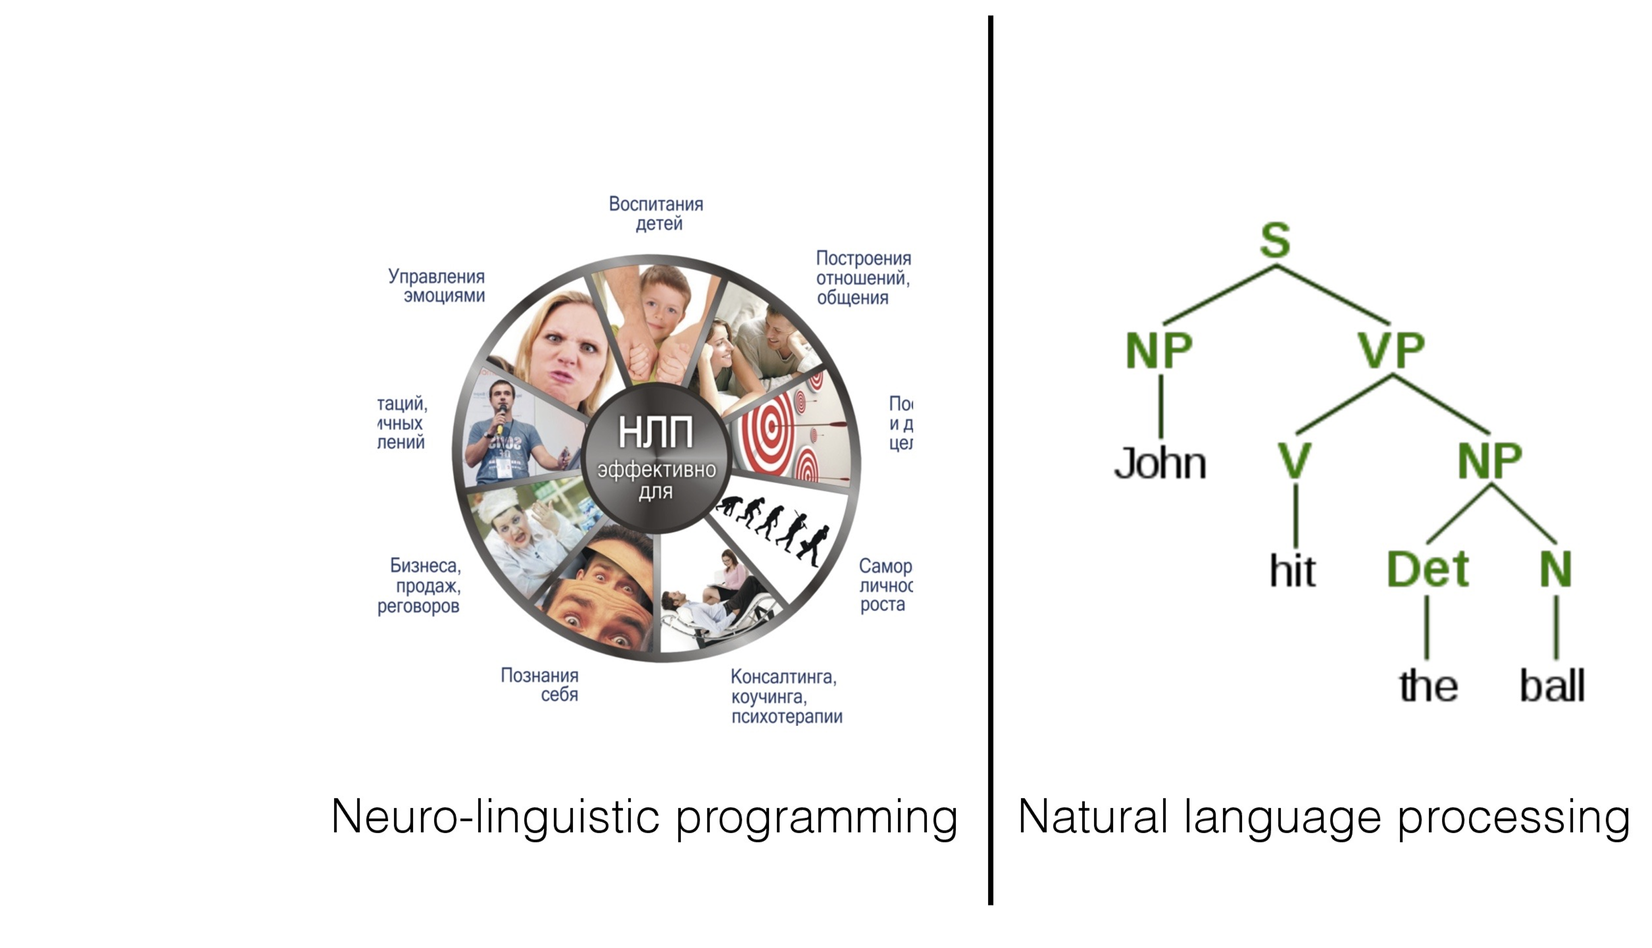
\includegraphics[width=0.83\paperwidth]{nlp3.png}}
	\begin{frame}
\end{frame}
}


{
	\usebackgroundtemplate{ 
		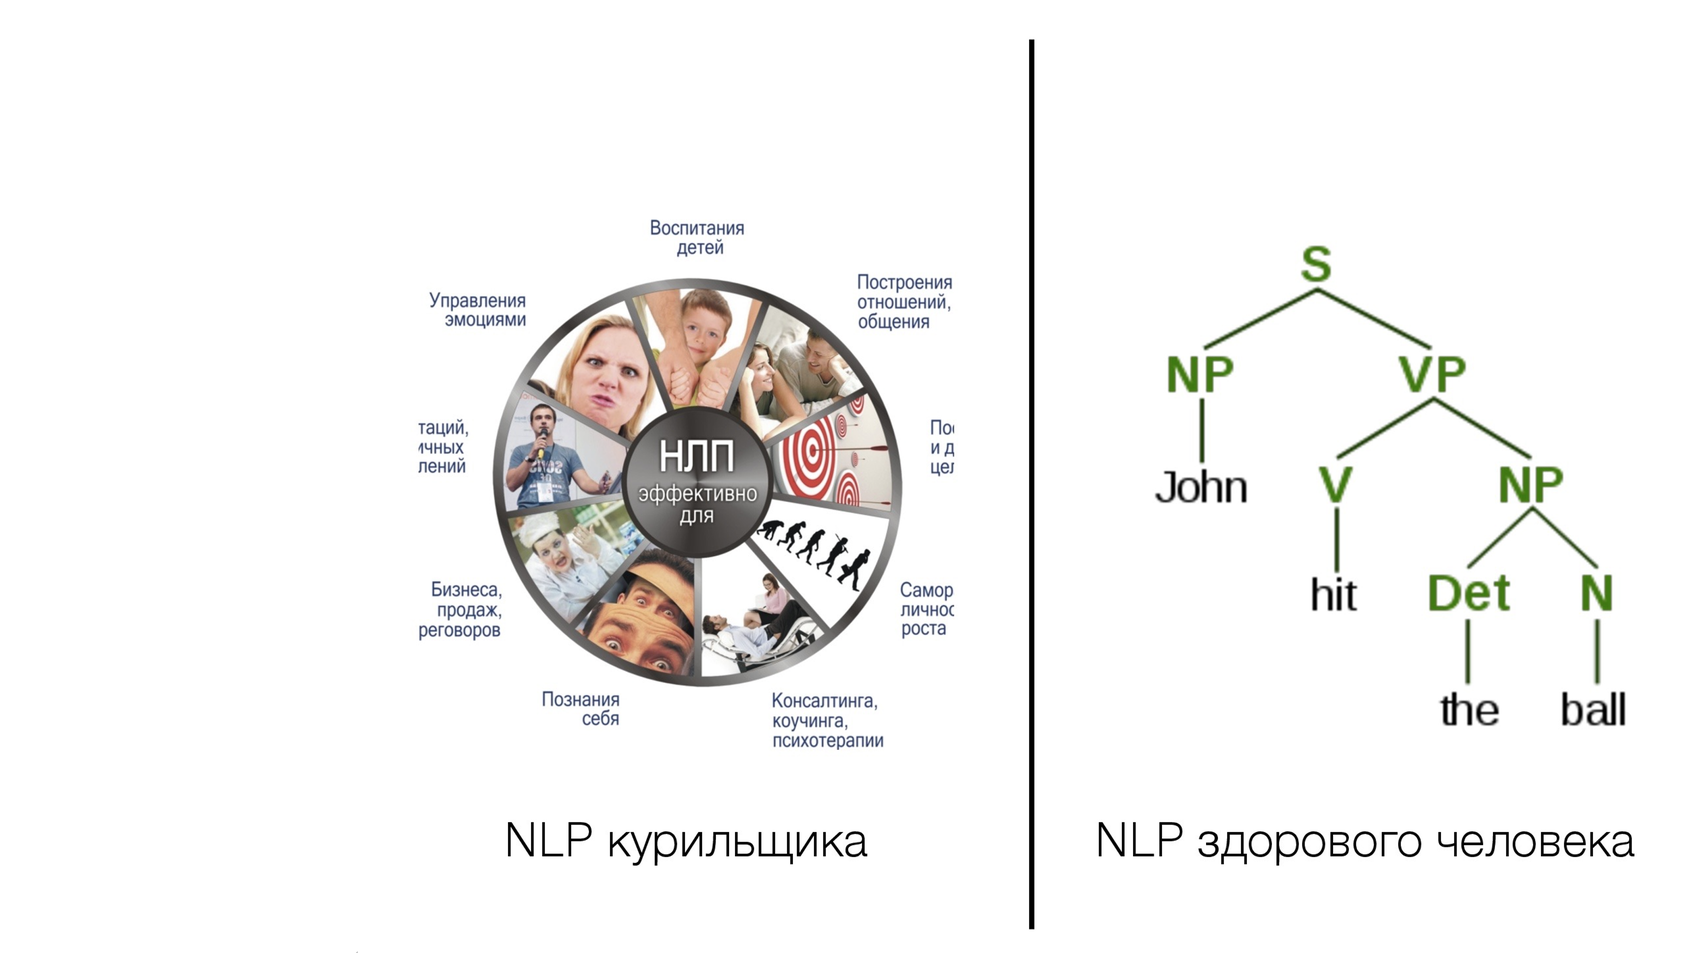
\includegraphics[width=0.83\paperwidth]{nlp4.png}}
	\begin{frame}
\end{frame}
}


\begin{frame}
\begin{block}{Классификация и регрессия:}
	\begin{itemize}
	\item Поиск спама
	\item Сентимент-анализ
	\item Модерация контента
	\item Предсказание популярности поста 
	\item Многое многое другое \ldots 
\end{itemize}
\end{block}

\begin{block}{Задачи посложнее:}
	\begin{itemize}
		\item Рекомендательные системы
		\item Диалоговые системы (чат боты)
		\item Машинный перевод 
		\item Тематизация новостей, их сжатие в краткое саммари
	\end{itemize}
\end{block}
\end{frame} 


\begin{frame}{Классификация текстов}
\begin{center}
	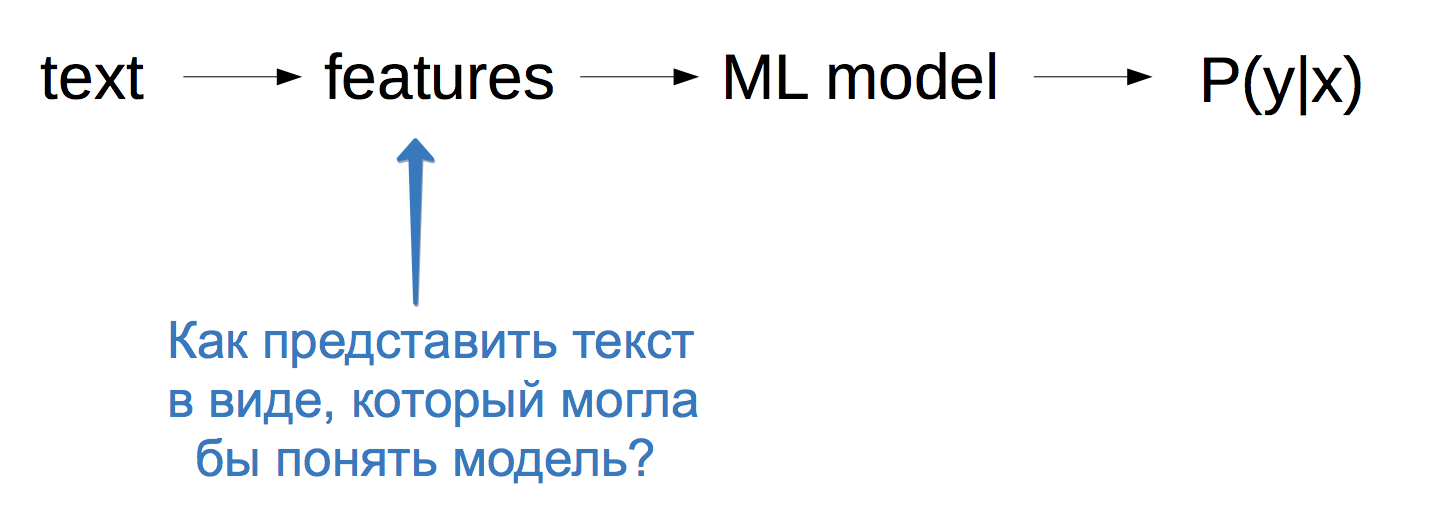
\includegraphics[width=.8\linewidth]{text1.png}
\end{center}
\end{frame} 


\begin{frame}{Что такое текст?}
\begin{columns}
\begin{column}{.48\linewidth}
	
\includegraphics[scale=0.3]{bender.png}
\end{column}

	\begin{column}{.48\linewidth}
\begin{wideitemize} 
	\item  Текст (документ) —  это последовательность токенов (слов)
	\item  Токен (слово) —  это последовательность символов
\end{wideitemize}
	\end{column}	
\end{columns}
\end{frame} 


\begin{frame}{Мешок слов}
\begin{center}
	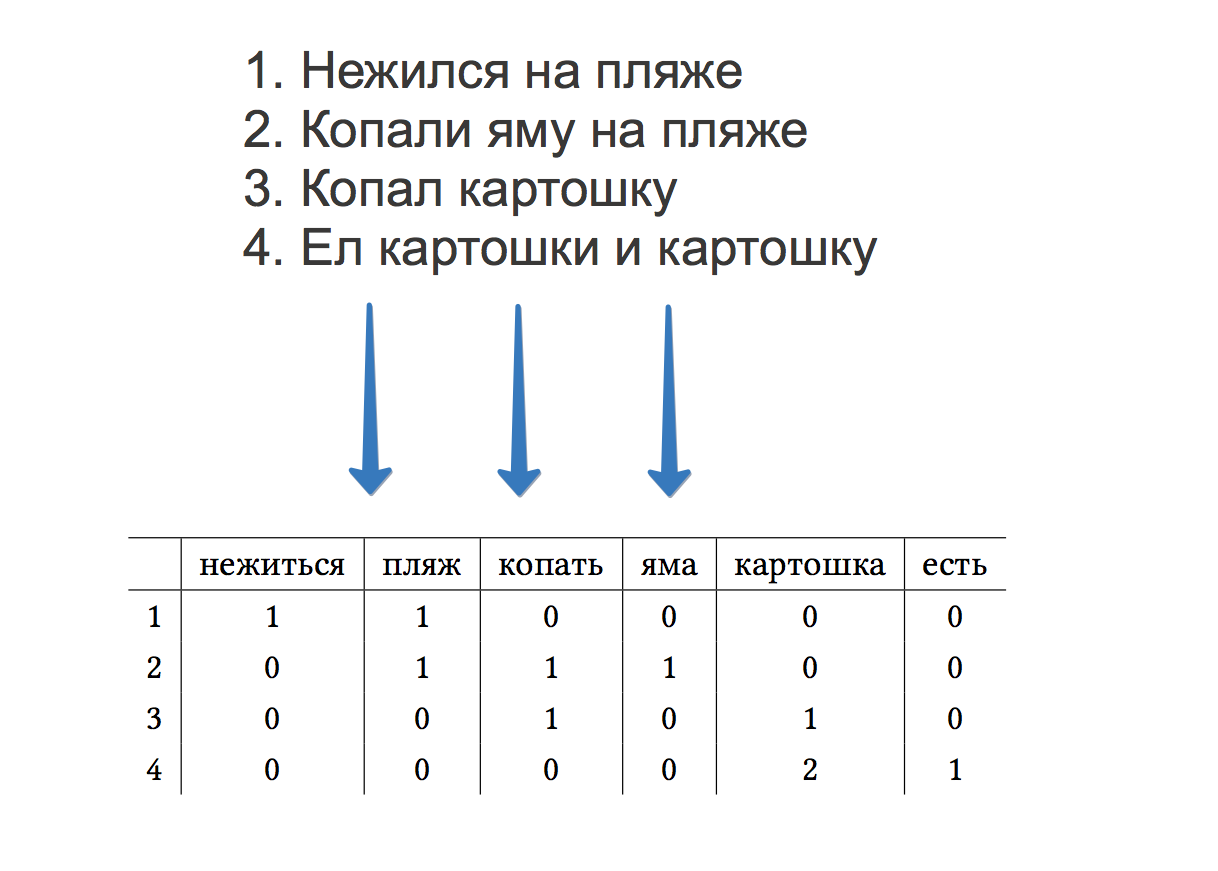
\includegraphics[width=.7\linewidth]{text.png}
\end{center}
\end{frame} 


\begin{frame}{Предобработка текста}
\begin{center}
	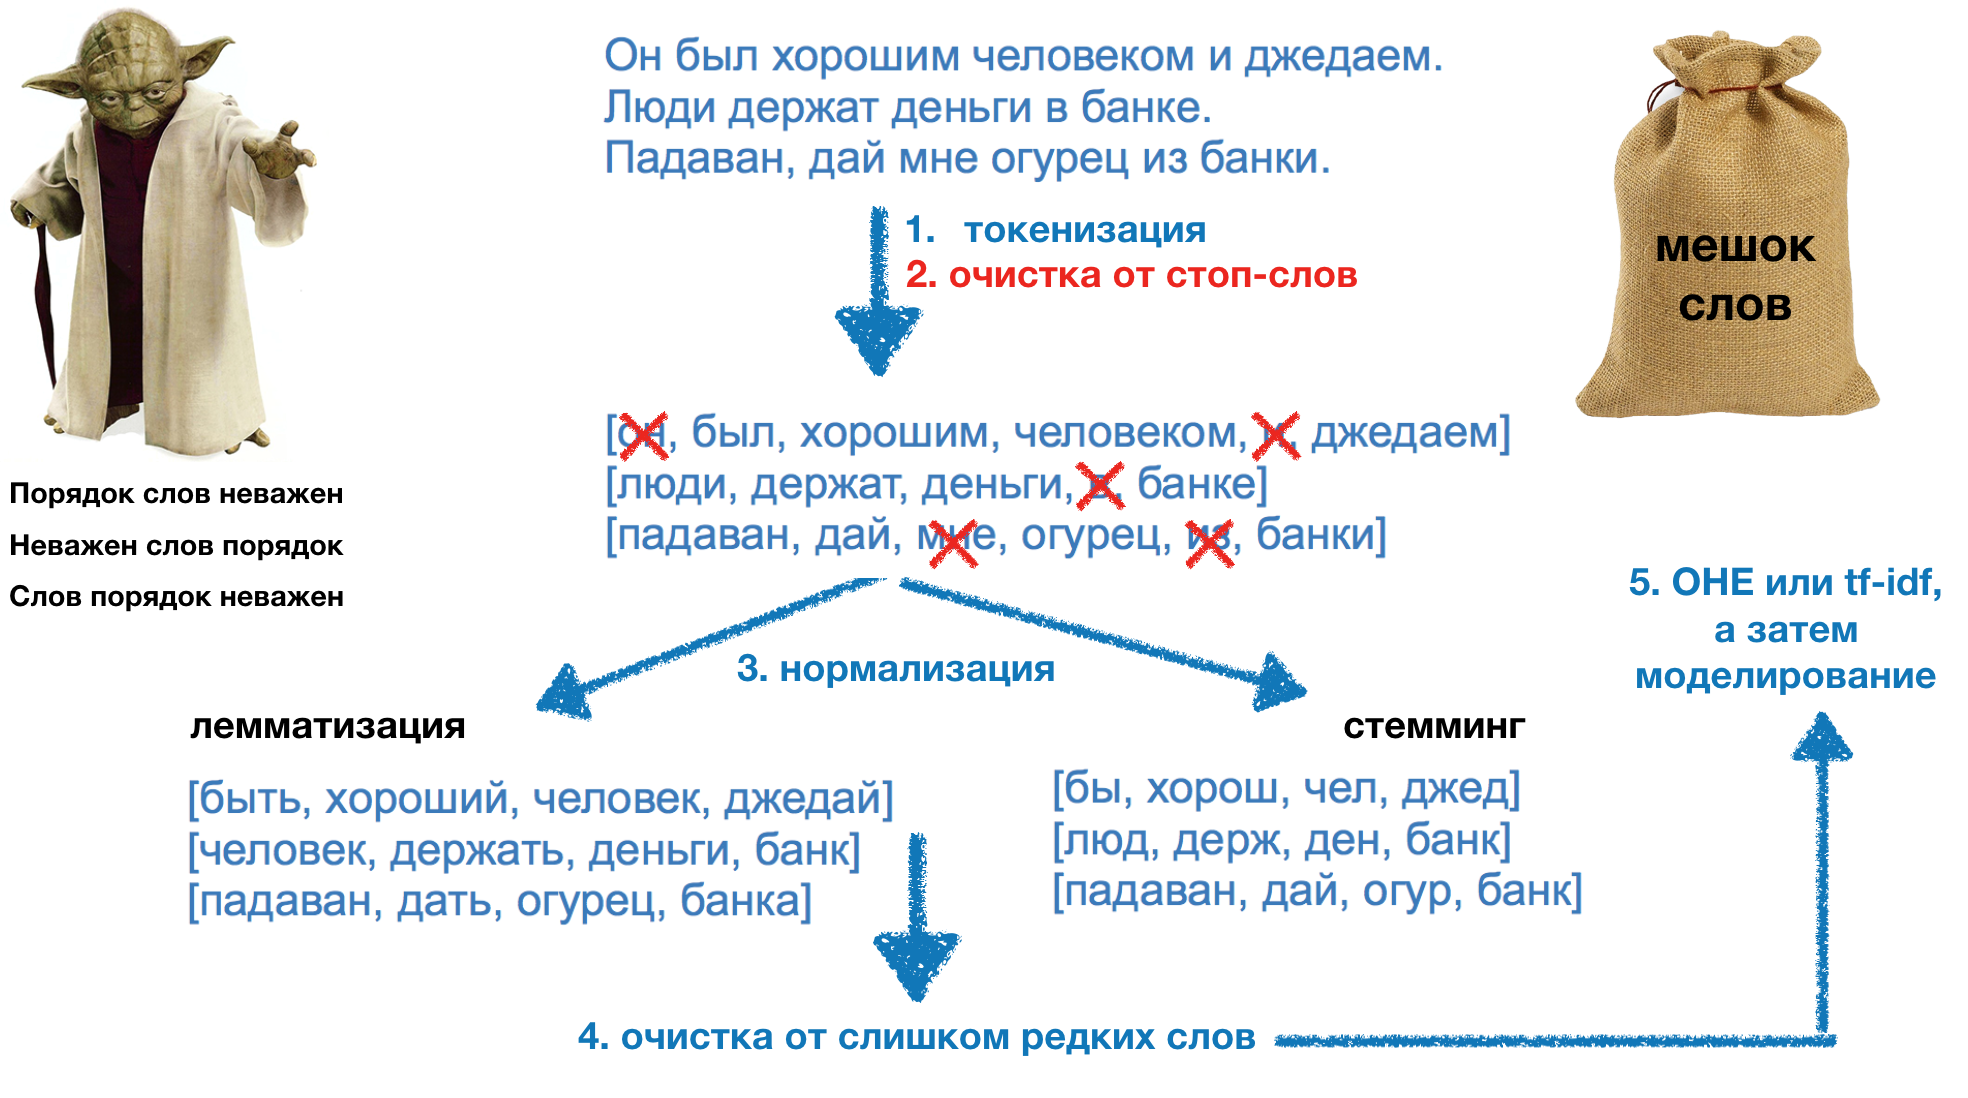
\includegraphics[width=.95\linewidth]{classic_text.png}
\end{center}
\end{frame} 

	

\begin{frame}{Ключевые мысли предыдущего слайда}
\begin{wideitemize} 
\item \textbf{Гипотеза мешка слов:} нам плевать на взаимное расположение слов. Порядок слов в предложении никак не сказывается на его смысле. 	{\color{red}  Следуя гипотезе, мы теряем часть информации.}
	
\item Рассматриваем каждое слово, как переменную $\Rightarrow$ большое пространство признаков. Нужно его урезать $\Rightarrow$ 	{\color{red}  Теряем ещё информацию.}

\item Хотим маленькое пространство признаков и много информации в нём!

\item \textbf{Дистрибутивная гипотеза:} слова с похожим смыслом будут встречаться в похожих контекстах.
\end{wideitemize}
\end{frame} 



\begin{transitionframe}
	\begin{center}
		\Huge  Из слов в вектора и обратно
	\end{center}
\end{transitionframe}


\begin{frame}{Words embeddings}
\begin{wideitemize} 
	\item \textbf{Наша цель:}  хотим научить компьютер понимать слова
	
	\item Идея! Давайте превратим наши слова в вектора размера $d$ и назовём их embeddings
	
	\item На вектора понакладываем хотелок! 
\end{wideitemize} 
\begin{center}
	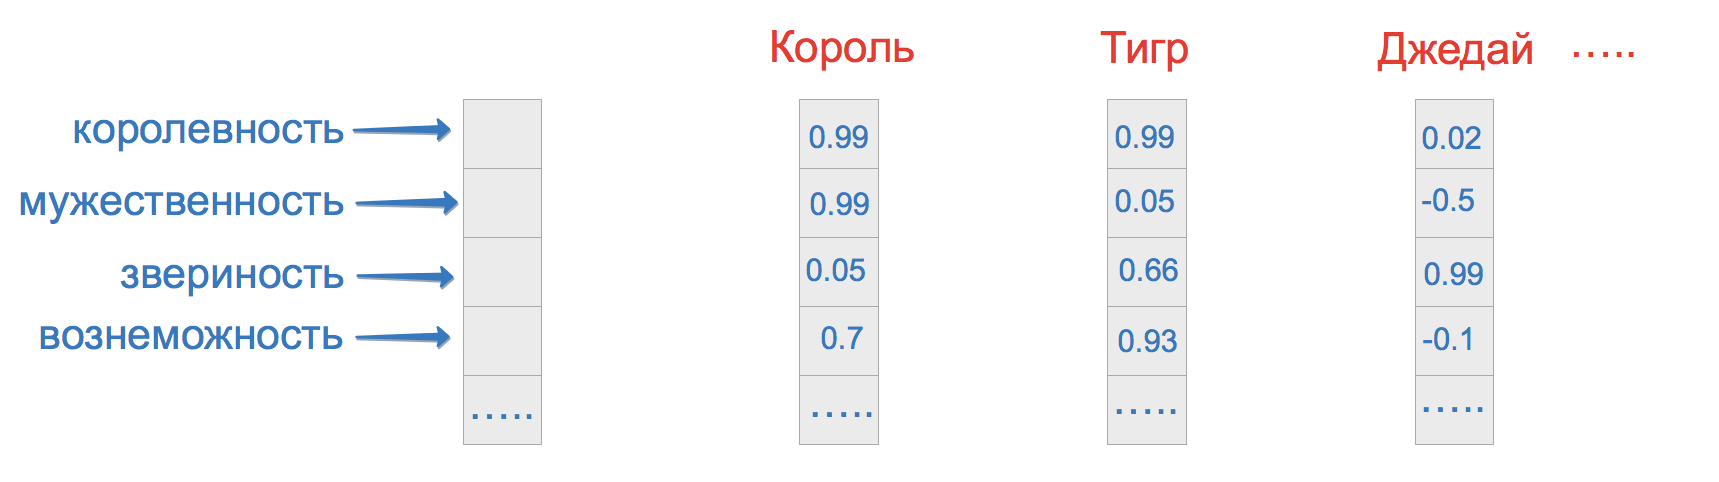
\includegraphics[width=.95\linewidth]{vectors.png}
\end{center}
\end{frame} 

\begin{frame}{Хотелка первая}
\begin{itemize} 
\item Хотим, чтобы модель улавливала семантические свойства слов
\end{itemize} 

\begin{center}
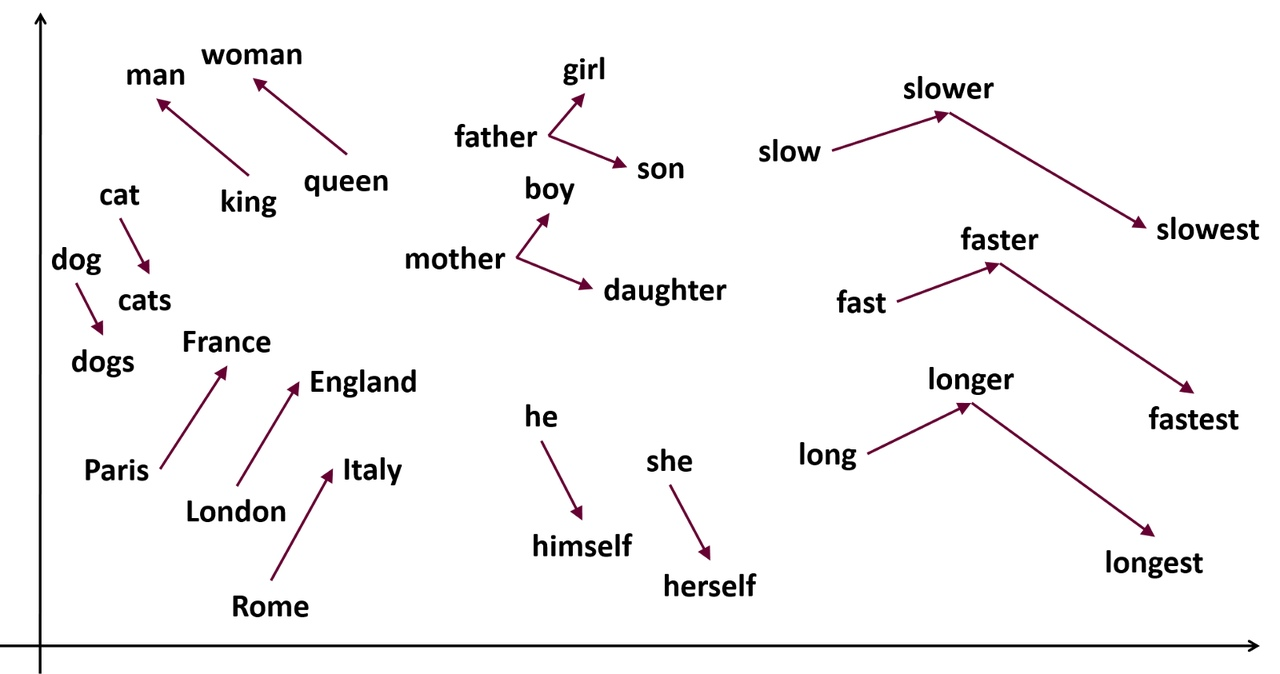
\includegraphics[width=.8\linewidth]{w2v_sim.jpg}
\end{center}
\end{frame} 


\begin{frame}{Хотелка вторая}
\begin{itemize} 
\item Модель понимала, где близкие по смыслу слова: кот, котёнок, кошка, тигр, лев, ...	
\end{itemize} 

\begin{center}
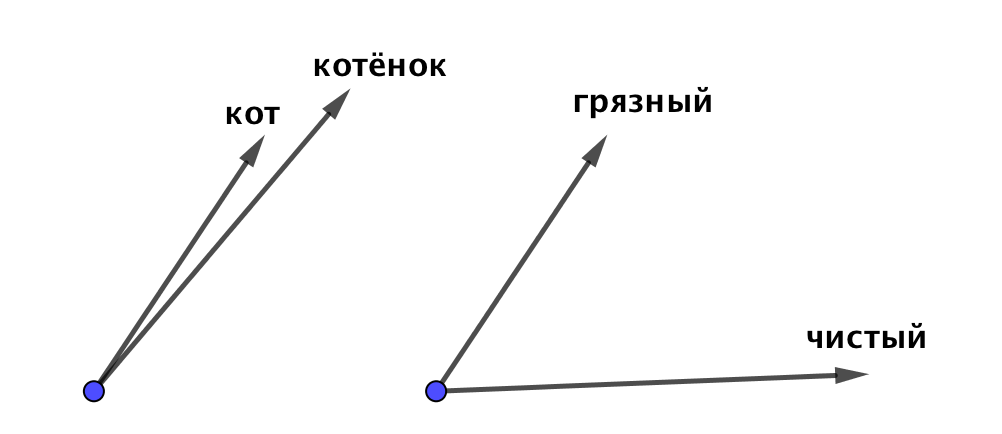
\includegraphics[width=.7\linewidth]{w2v_dist.png}
\end{center}
\end{frame} 


\begin{frame}{Хотелка третья}
\begin{itemize} 
\item Арифметика! 
\end{itemize} 

\begin{center}
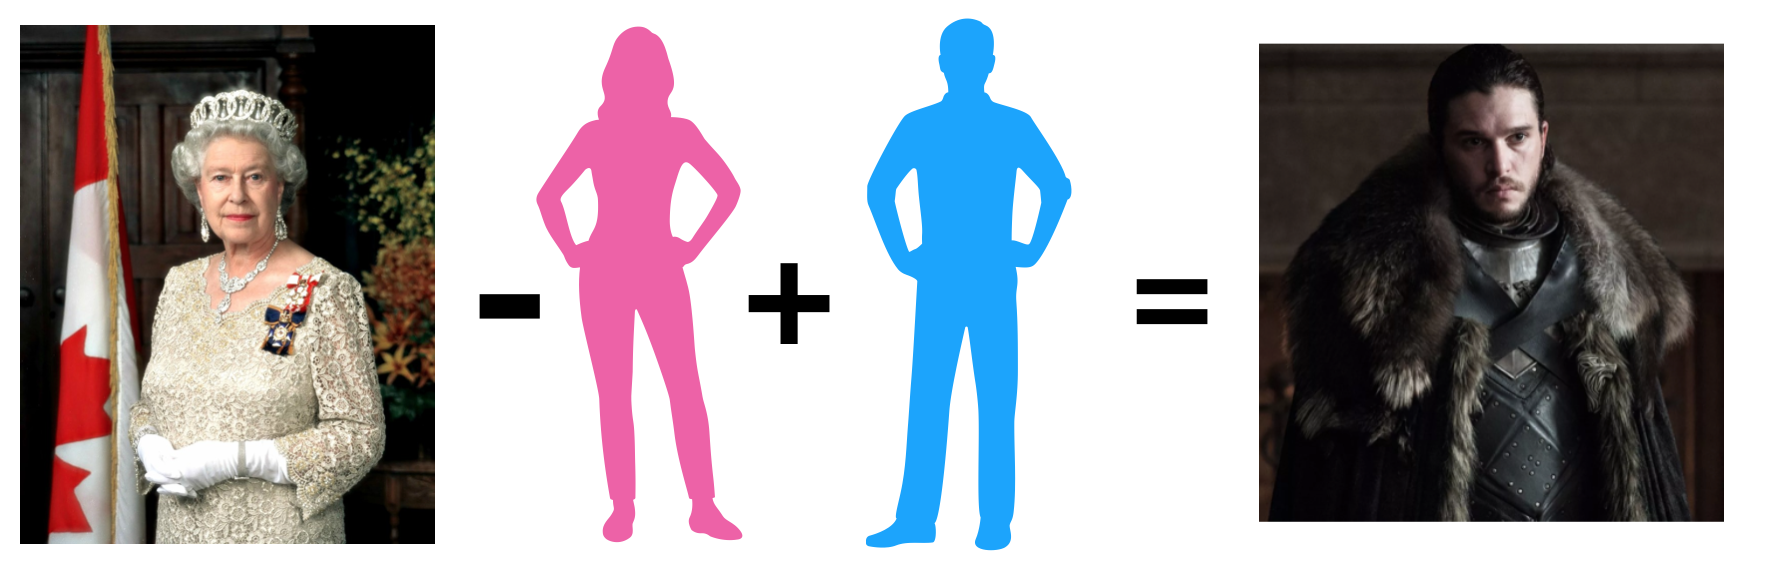
\includegraphics[width=.8\linewidth]{w2v_arith.png}
\end{center}
\end{frame} 



\begin{frame}{Томаш Миколов}
\begin{columns}[T] 
\begin{column}{.4\textwidth}
\begin{wideitemize} 
\item Звучит как магия, но работает

\item  В 2013 году модель предложена чешским аспирантом  Томашем Миколовым

\item После работал в Google, сейчас ушёл в Facebook  
\end{wideitemize} 
\end{column}%
\hfill%
\begin{column}{.6\textwidth}
\begin{center}
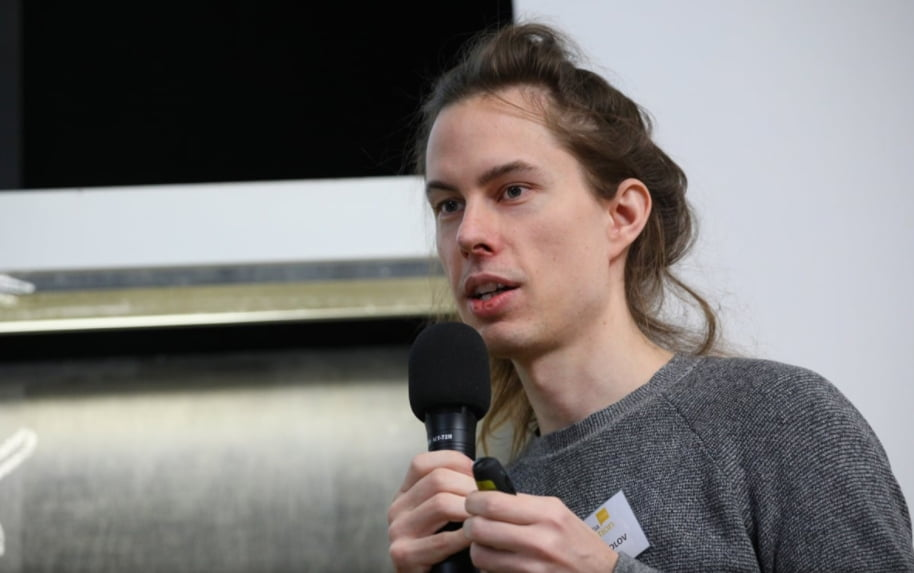
\includegraphics[width=.99\linewidth]{tomas-mikolov.jpg}
\end{center}
\end{column}%
\end{columns}
\end{frame}


% \begin{frame}{Расстояния между векторами}
% \end{frame} 

\begin{frame}{Постановка задачи}
\begin{center}
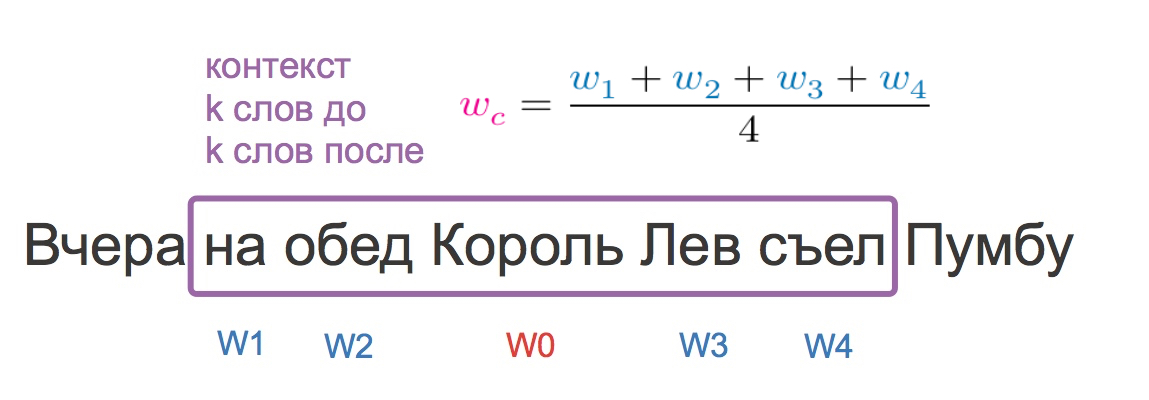
\includegraphics[width=.7\linewidth]{context_1.jpg}
\end{center}
\begin{itemize} 
\item \textbf{Контекст} — $k$ слов до рассматриваемого и $k$ после него. 

%{ 	\[ {\color{magenta} w_c } = \frac{ {\color{blue} w_1 } + {\color{blue} w_2} + {\color{blue} w_3} + {\color{blue} w_4 }}{4} \] }

\item Вероятность встретить наше слово в контексте $c$: 

\[
P(w_0 \mid w_c) = \frac{e^{s(w_0, w_c)}}{\sum e^{s(w_i, w_c)}}
\]

\end{itemize} 
\end{frame} 


\begin{frame}{Максимально правдоподобно}
\begin{wideitemize} 
\item Вероятность встретить наше слово в контексте $c$: 

\[
P(w_0 \mid w_c) = \frac{e^{s(w_0, w_c)}}{\sum e^{s(w_i, w_c)}}
\]

\item Мы хотим настроить вектора для слов так, чтобы эти вероятности были большими, если слово встречается в контексте и маленькими, если не встречаются. 

\item Воспользуемся методом максимального правдоподобия: 

\[ 
\ln L = \sum_{(i,c)} \ln P(w_i \mid w_c)  \to \max_{w}.
\]
\end{wideitemize} 
\end{frame} 

\begin{frame}{Проблемы}
\begin{wideitemize} 
\item Очень много параметров $W$. По каждому брать производную?! 

\item Хочется побыстрее. Любая взвешенная сумма - нейросеть. Давайте запишем правдоподобие в виде нейросетки.

\item Есть два подхода: CBOW (непрерывный мешок слов). В нём мы по заданному контексту слова пытаемся предсказать слово.

\item Skip-gram — по заданному слову пытаемся предсказать его контекст 
\end{wideitemize} 
\end{frame} 


\begin{frame}{CBOW}
\begin{center}
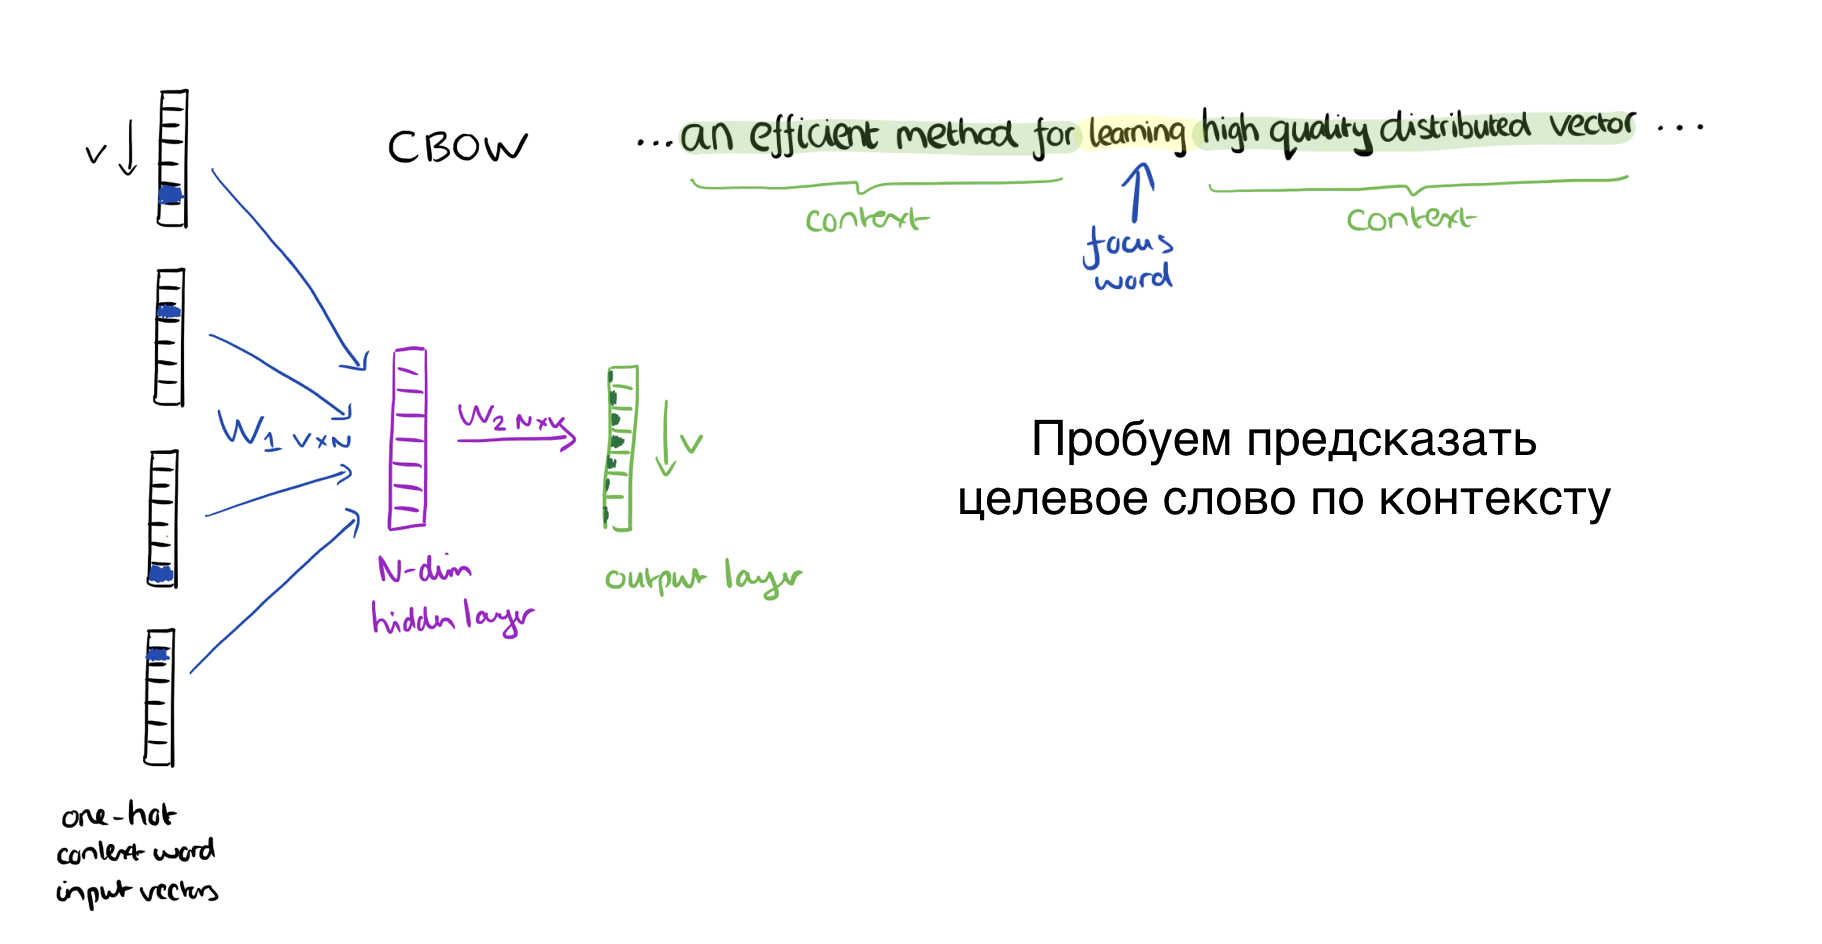
\includegraphics[width=.95\linewidth]{CBOW.png}
\end{center}
\end{frame} 


\begin{frame}{Skip-gram}
\begin{center}
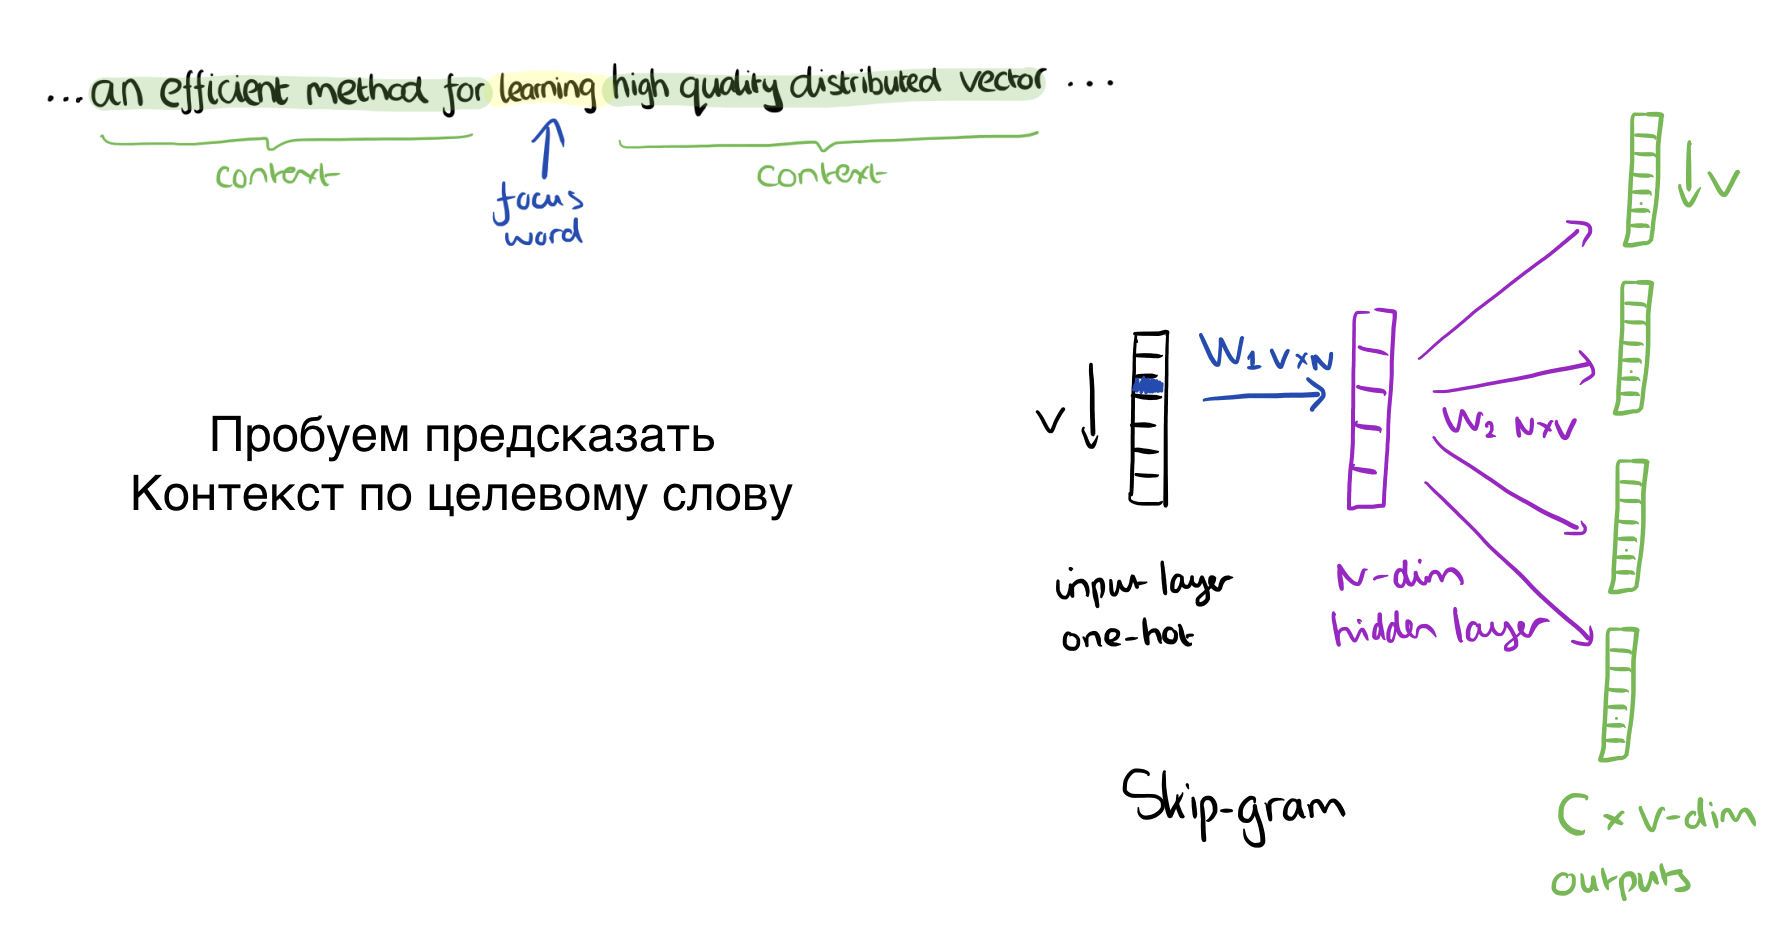
\includegraphics[width=.95\linewidth]{skipgram.png}
\end{center}
\end{frame} 


\begin{frame}{Word2Vec}
\begin{wideitemize} 
	\item  Трансформирует пространство текстов в $d$-мерное пространство векторов
	\item  В матрице $W_1$ будут записаны наши итоговые вектора
	\item  Между словами на выходе выполняются интересные арифметические свойства 
	\item  Для обучения требует много данных 
\end{wideitemize} 
\end{frame} 


\begin{frame}{Откуда взять данные (дампы Википедии)}
\begin{center}
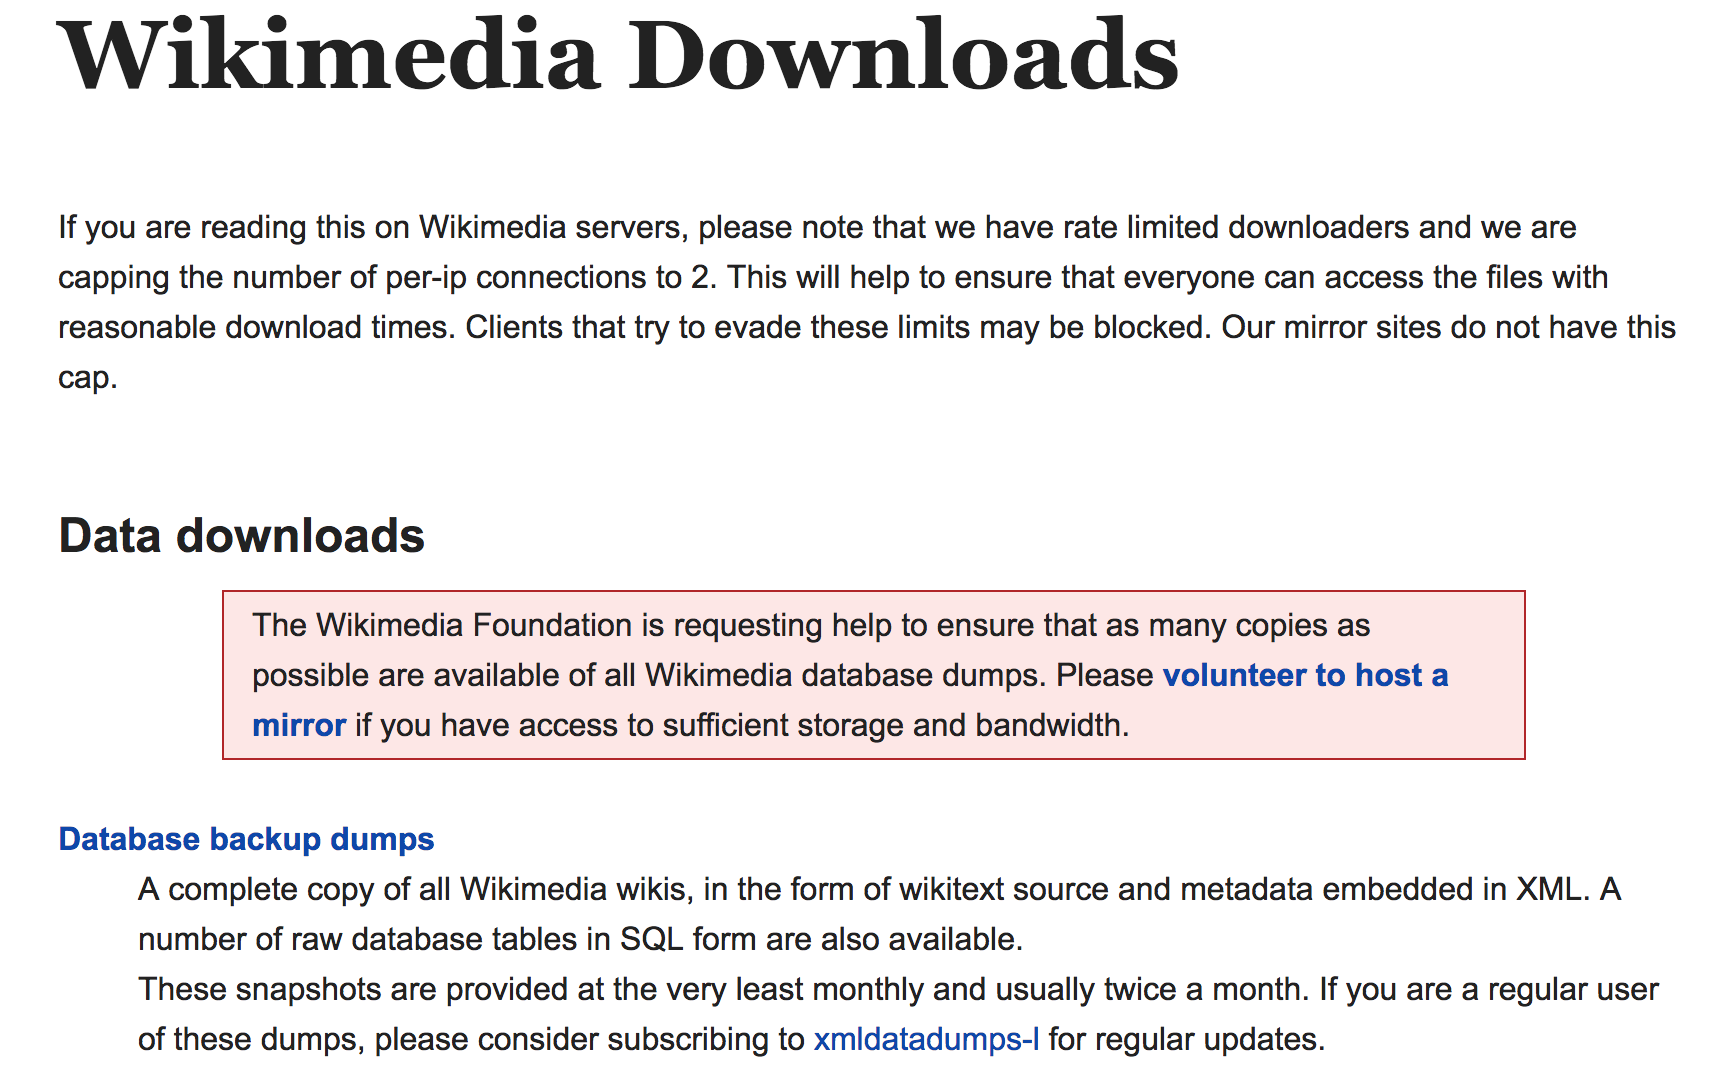
\includegraphics[width=.7\linewidth]{wiki_dumps.png}
\end{center}

\vfill

\footnotesize Дампы википедии для разных языков:  {\color{blue} \url{https://dumps.wikimedia.org}} \newline Например, для русского:  {\color{blue} \url{https://dumps.wikimedia.org/ruwiki/}} 
\end{frame} 


\begin{frame}{Откуда взять данные (НКРЯ)}
\begin{center}

\includegraphics[width=.99\linewidth]{ruscorp.png}
\end{center}

\vfill

\footnotesize Национальный корпус Русского языка:  {\color{blue} \url{http://ruscorpora.ru}} 
\end{frame} 


\begin{frame}{Где взять уже готовенькое (проект RusVectōrēs)}
\begin{center}
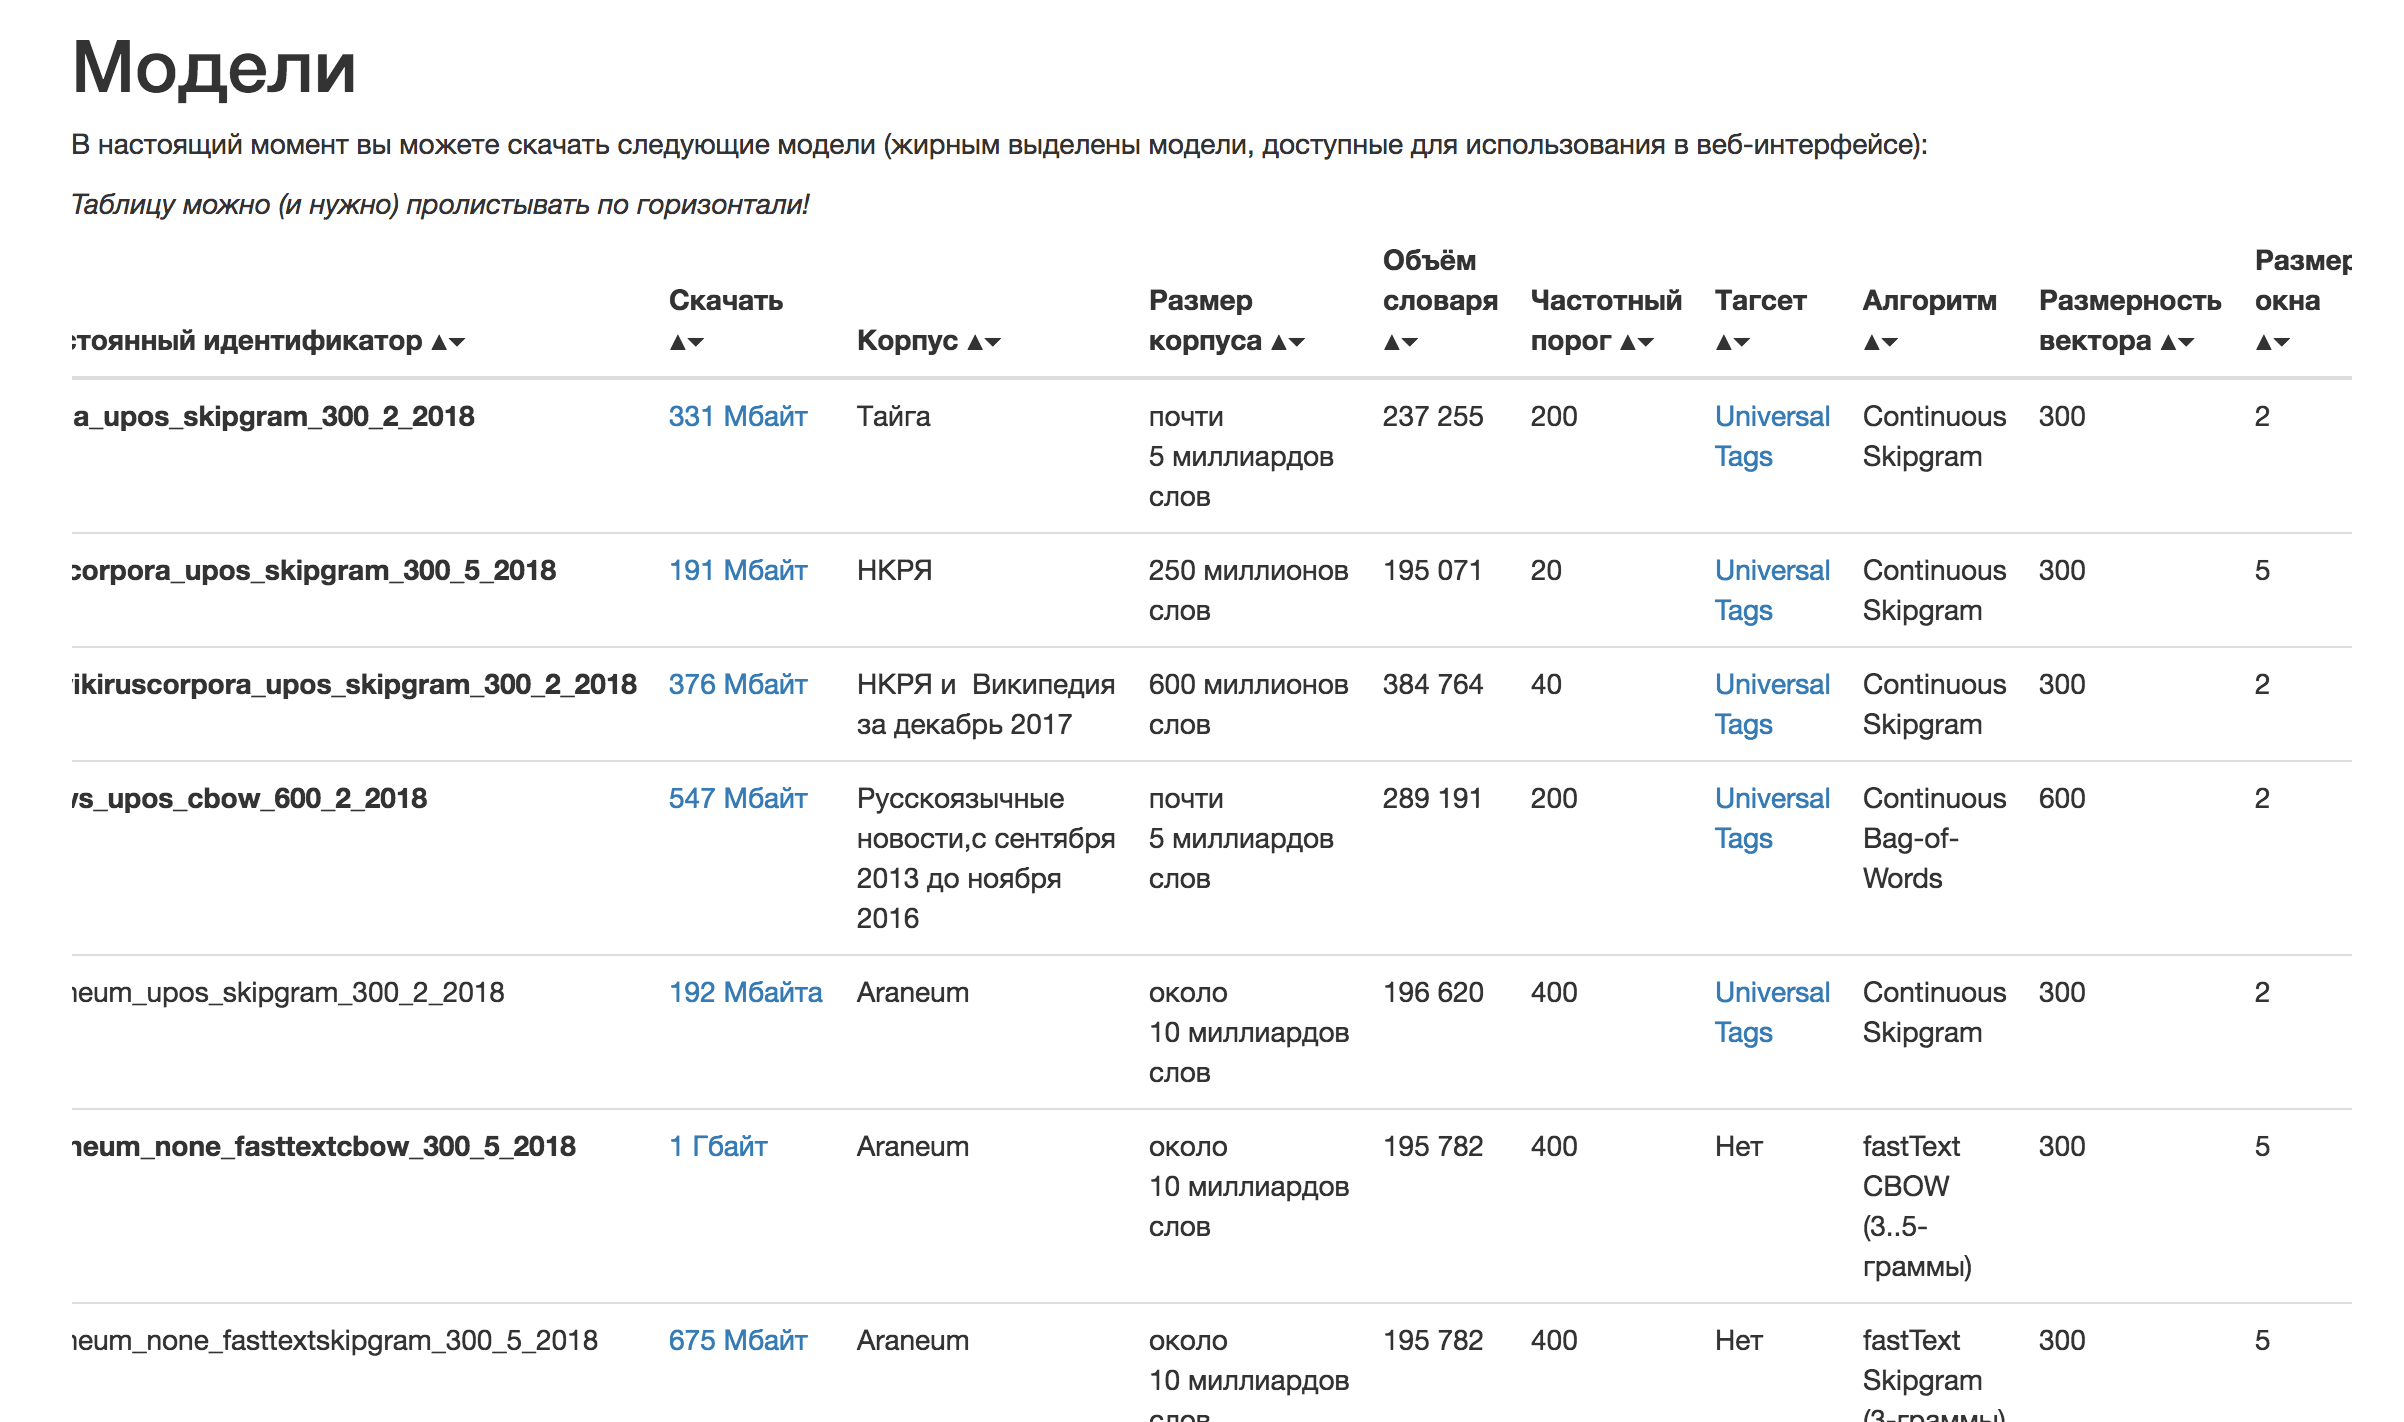
\includegraphics[width=.7\linewidth]{rusvec_models.png}
\end{center}

\vfill

\footnotesize Куча разных моделей для русского языка:  {\color{blue} \url{https://rusvectores.org/ru/models/}}
\end{frame} 


\begin{frame}{Где взять уже готовенькое (проект RusVectōrēs)}
\begin{center}
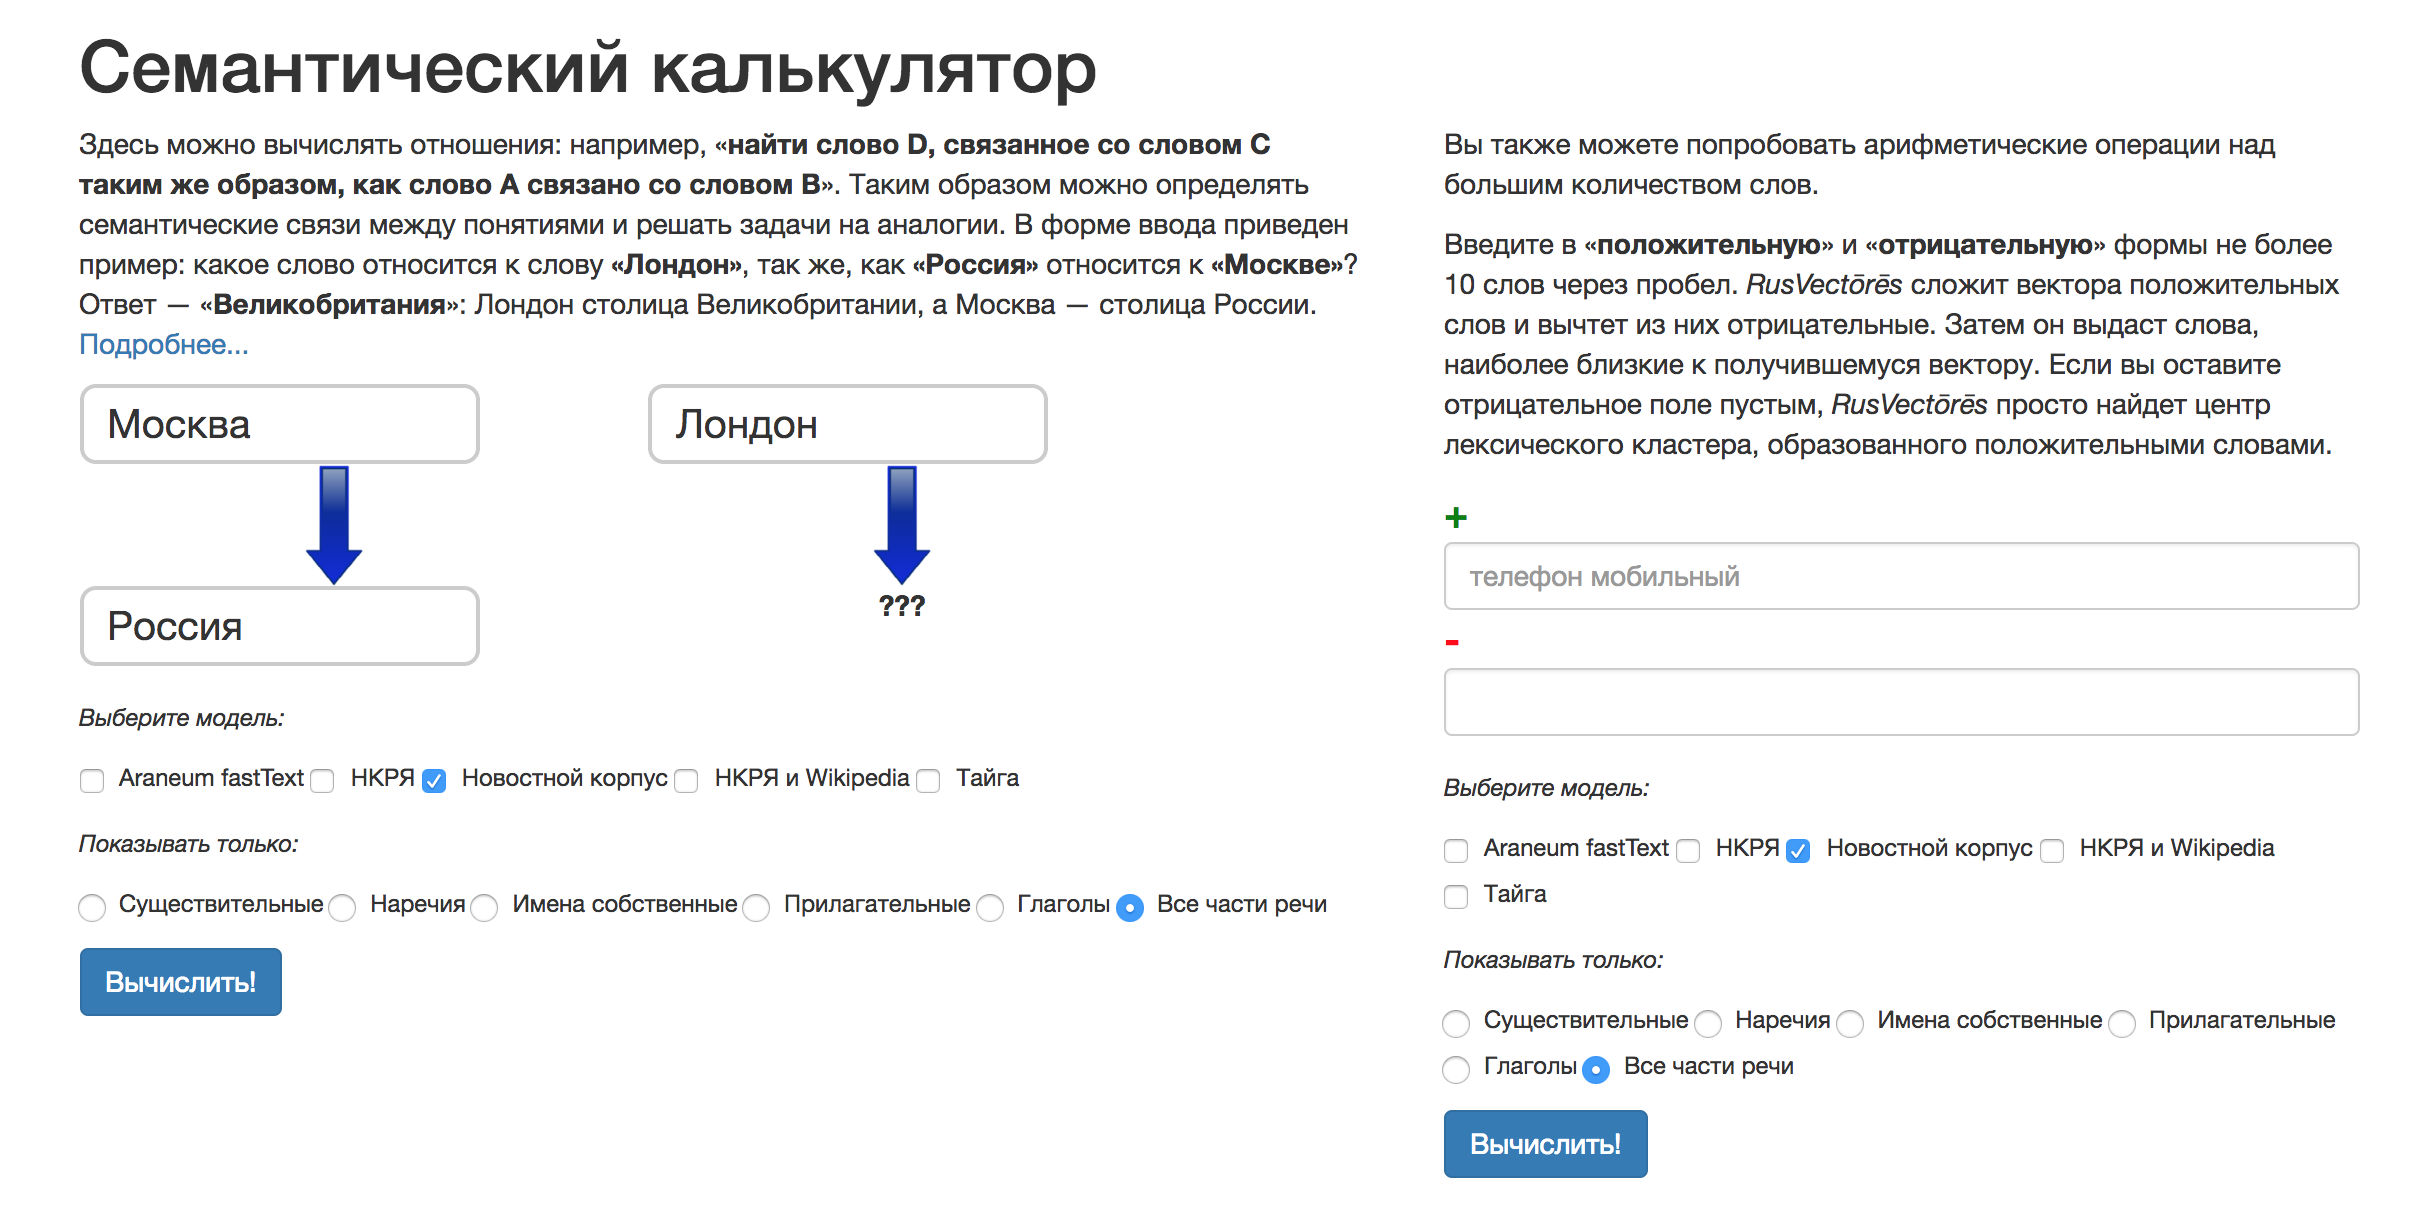
\includegraphics[width=.65\linewidth]{rusvec_calc.png}
\end{center}

\vfill

\footnotesize Куча разных моделей для русского языка:  {\color{blue} \url{https://rusvectores.org/ru/calculator/}}
\end{frame} 


\begin{frame}{Где взять уже готовенькое (Google)}
\begin{center}
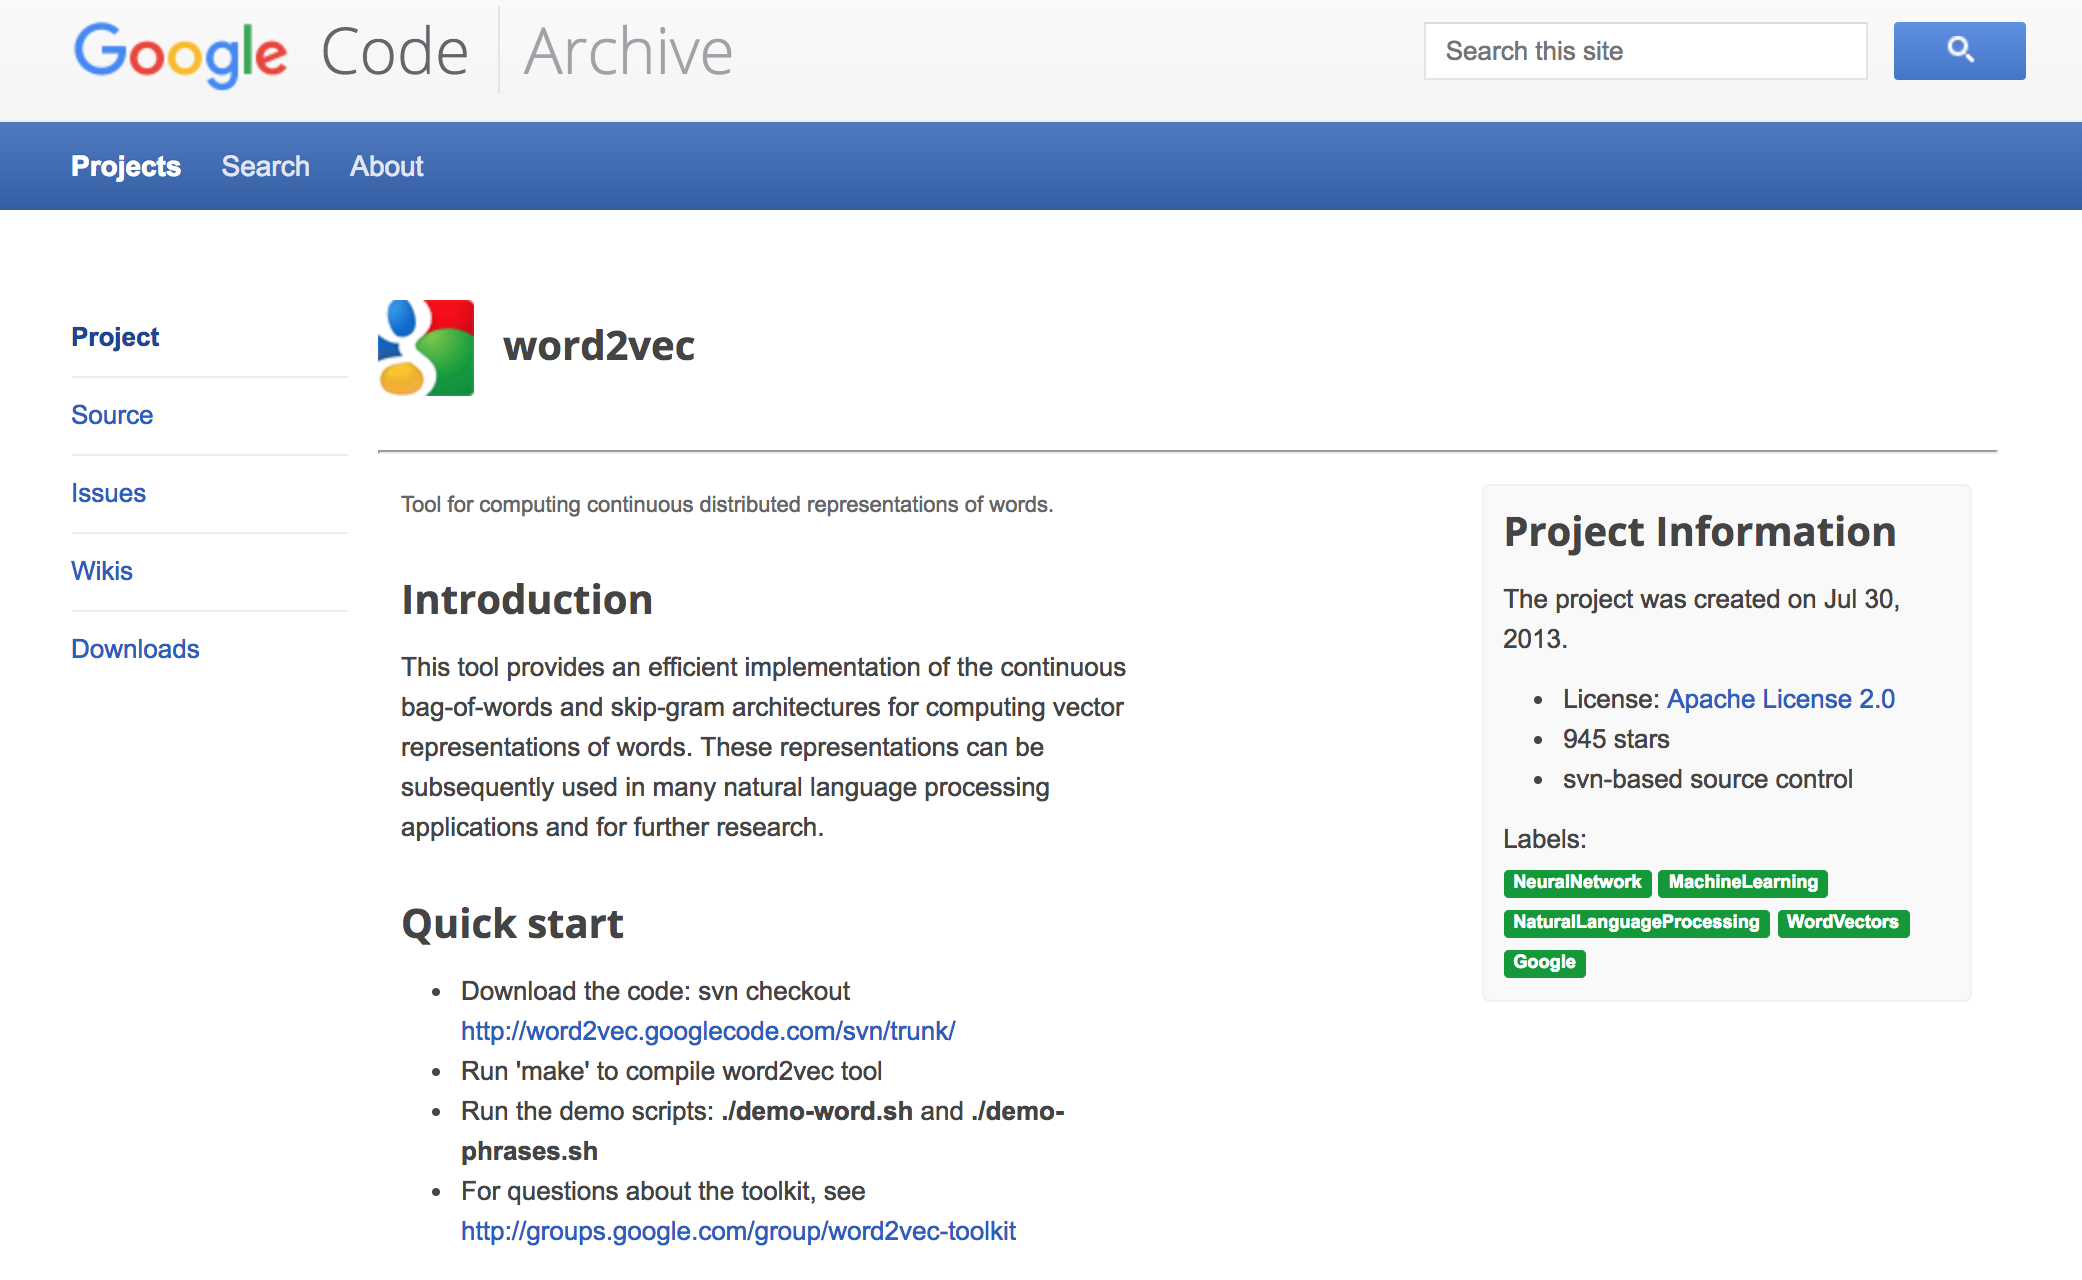
\includegraphics[width=.65\linewidth]{google_wv.png}
\end{center}

\vfill

\footnotesize Гугловская модель для английского языка:  {\color{blue} \url{https://code.google.com/archive/p/word2vec/}}
\end{frame} 



\begin{frame}{Полезные мысли}
\begin{itemize} 
	\item В tensorflow довольно легко собрать свой собственный w2v и обучить его, но не стоит делать это.  Ваша реализация не будет такой эффективной, как уже существующие специализированные реализации. За последние годы алгоритмы для обучения w2v претерпели существенную эволюцию. 
	
	\item   Реализация w2v из пакета gensim зачастую работает быстрее, чем модели, написанные в стандартных для нейросеток бэкэндах. Это происходит из-за многопоточности и разных умных оптимизаций тонких мест в обучении. 
	
	\item  При достаточно большом корпусе текстов можно не делать лемматизацию. Сетка сама поймёт по контексту, что слова близки и присвоит им похожие вектора.
	
	\item Если у вас специфическая задача, в которой встречается специфическая лексика, возьмите предобученную на большом корпусе сетку и дообучите её под свои нужды.
\end{itemize} 
\end{frame} 


\begin{transitionframe}
\begin{center}
\Huge Попробуем обучить свою модель и сравнить её с RusVectōrēs моделью
\end{center}
\end{transitionframe}


\begin{transitionframe}
	\begin{center}
		\Huge Нейросетки для текстов
	\end{center}
\end{transitionframe}


\begin{frame}{Нейросеть для текстов}
\begin{center}
	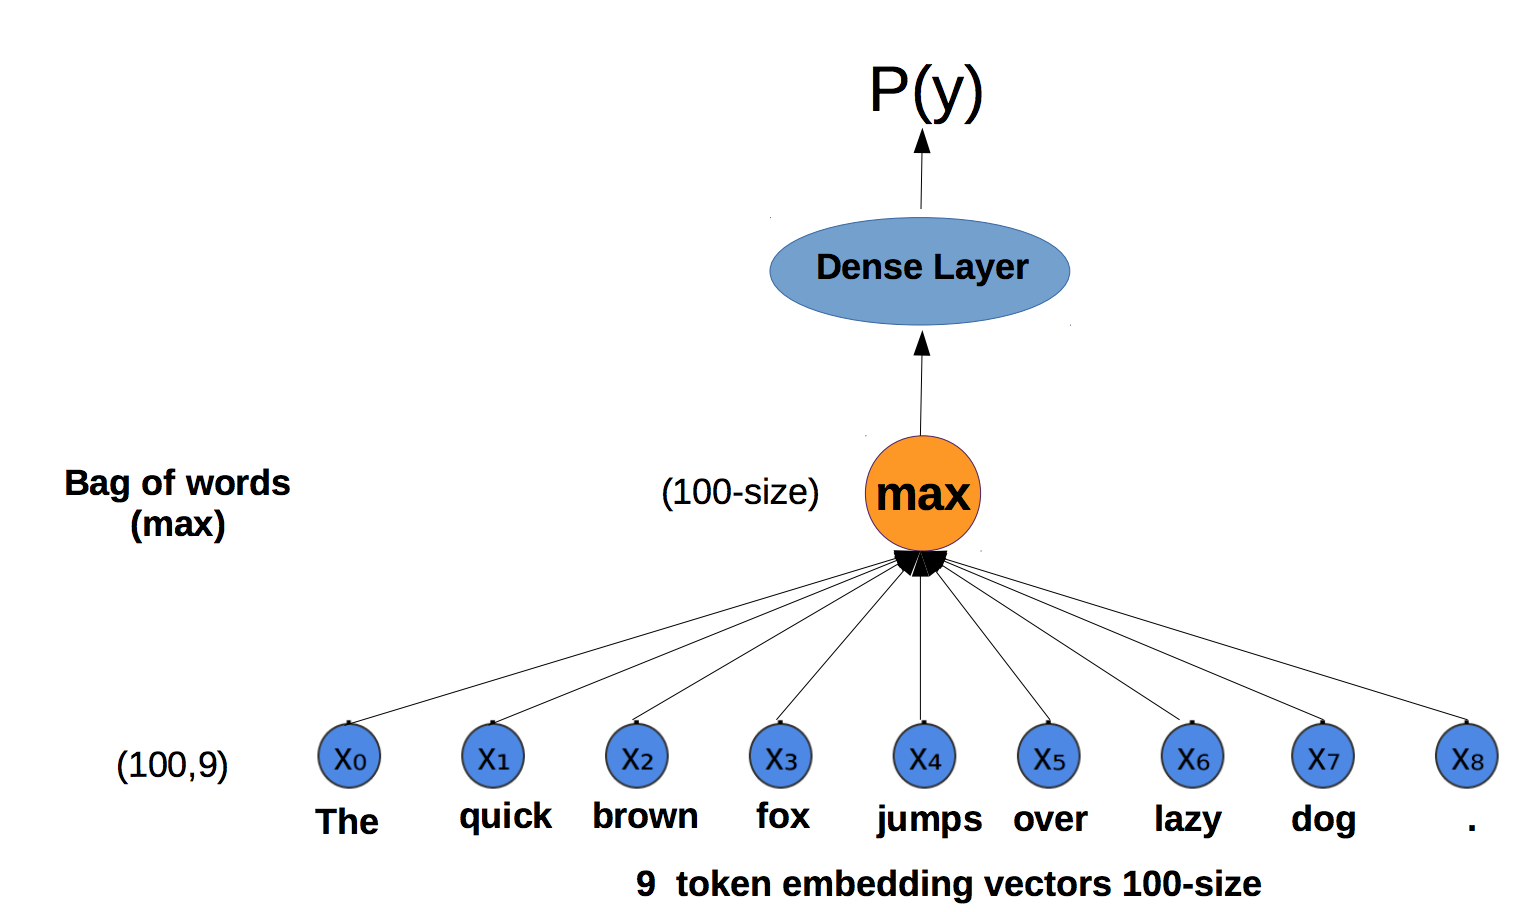
\includegraphics[width=.75\linewidth]{text_nn.png}
\end{center}
\end{frame} 


\begin{frame}{Проблемы}
\begin{wideitemize} 
	\item  Теряем информацию о порядке слов 
	\item  Решить эту проблему можно обучив эмбединги для биграм, трграм и тд, но это расширит пространство признаков
	\item  Можно решить эту проблему с помощью рекурентных нейросеток, о них мы будем говорить в следущий раз 
	\item  \alert{Можно решить эту проблему с помощью свёрточного слоя}
\end{wideitemize} 
\end{frame} 


\begin{frame}{Свёрточная сетка}
\begin{center}
	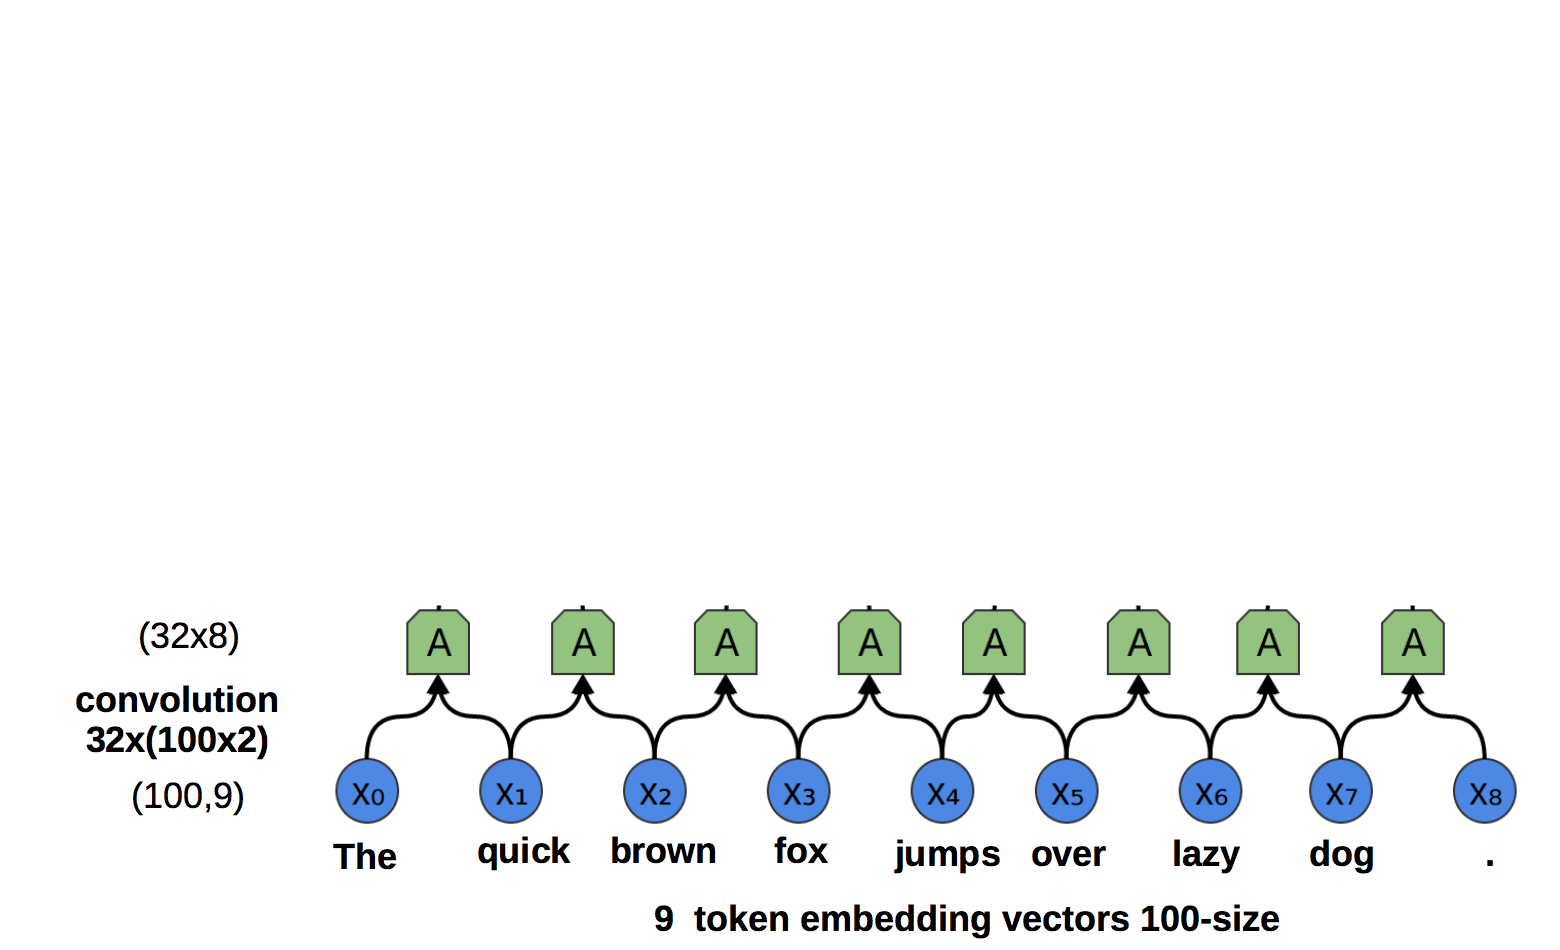
\includegraphics[width=.75\linewidth]{conv1.png}
\end{center}
\end{frame} 


\begin{frame}{Свёрточная сетка}
\begin{center}
	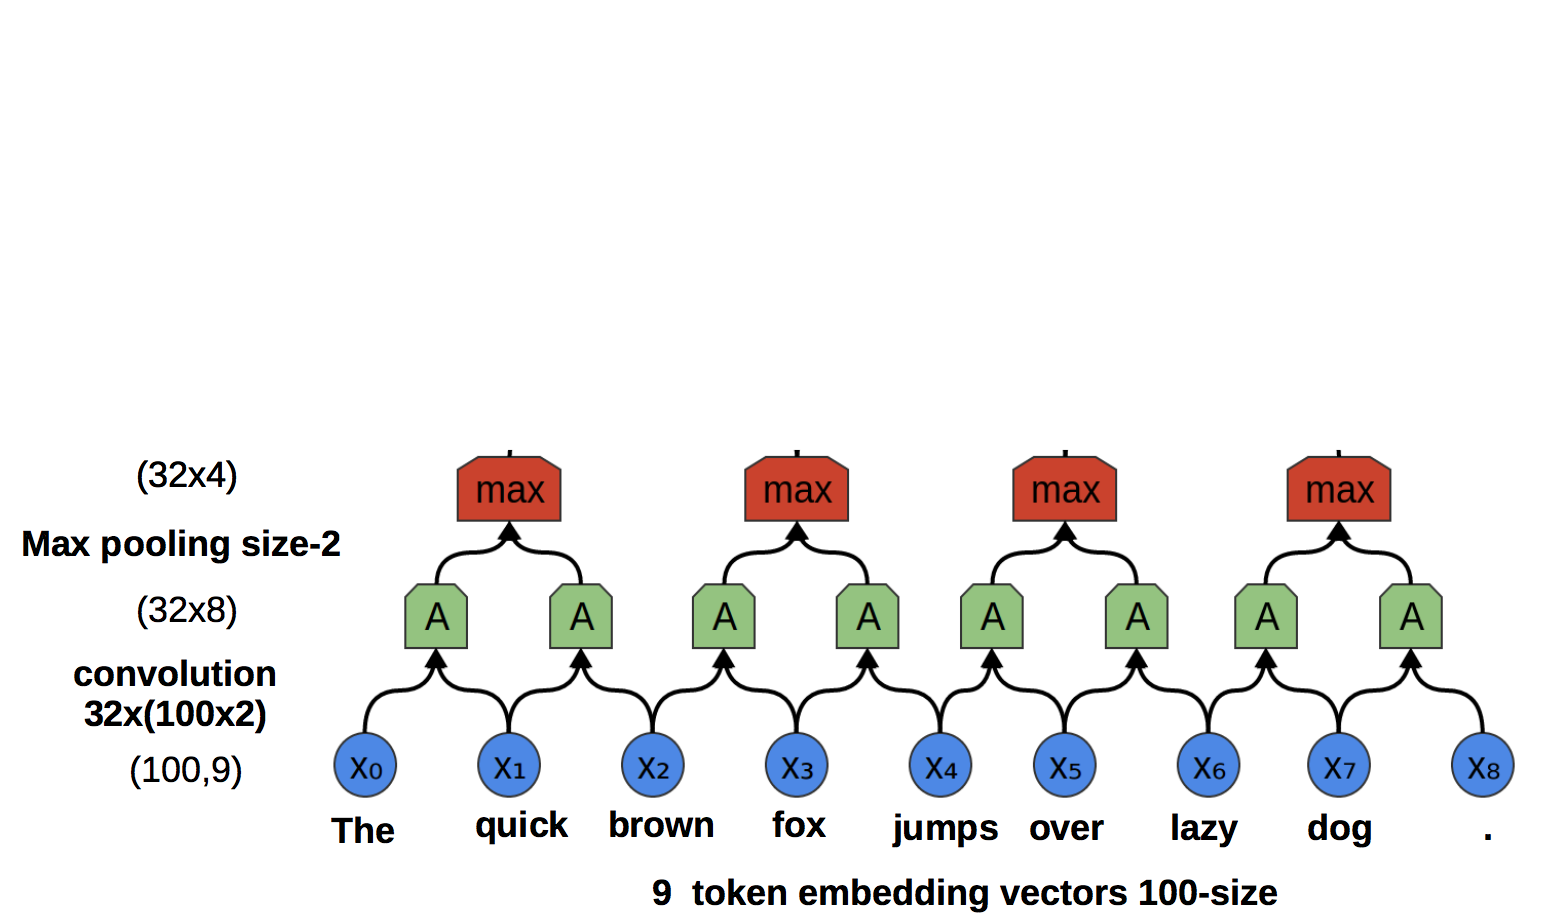
\includegraphics[width=.75\linewidth]{conv2.png}
\end{center}
\end{frame} 


\begin{frame}{Свёрточная сетка}
\begin{center}
	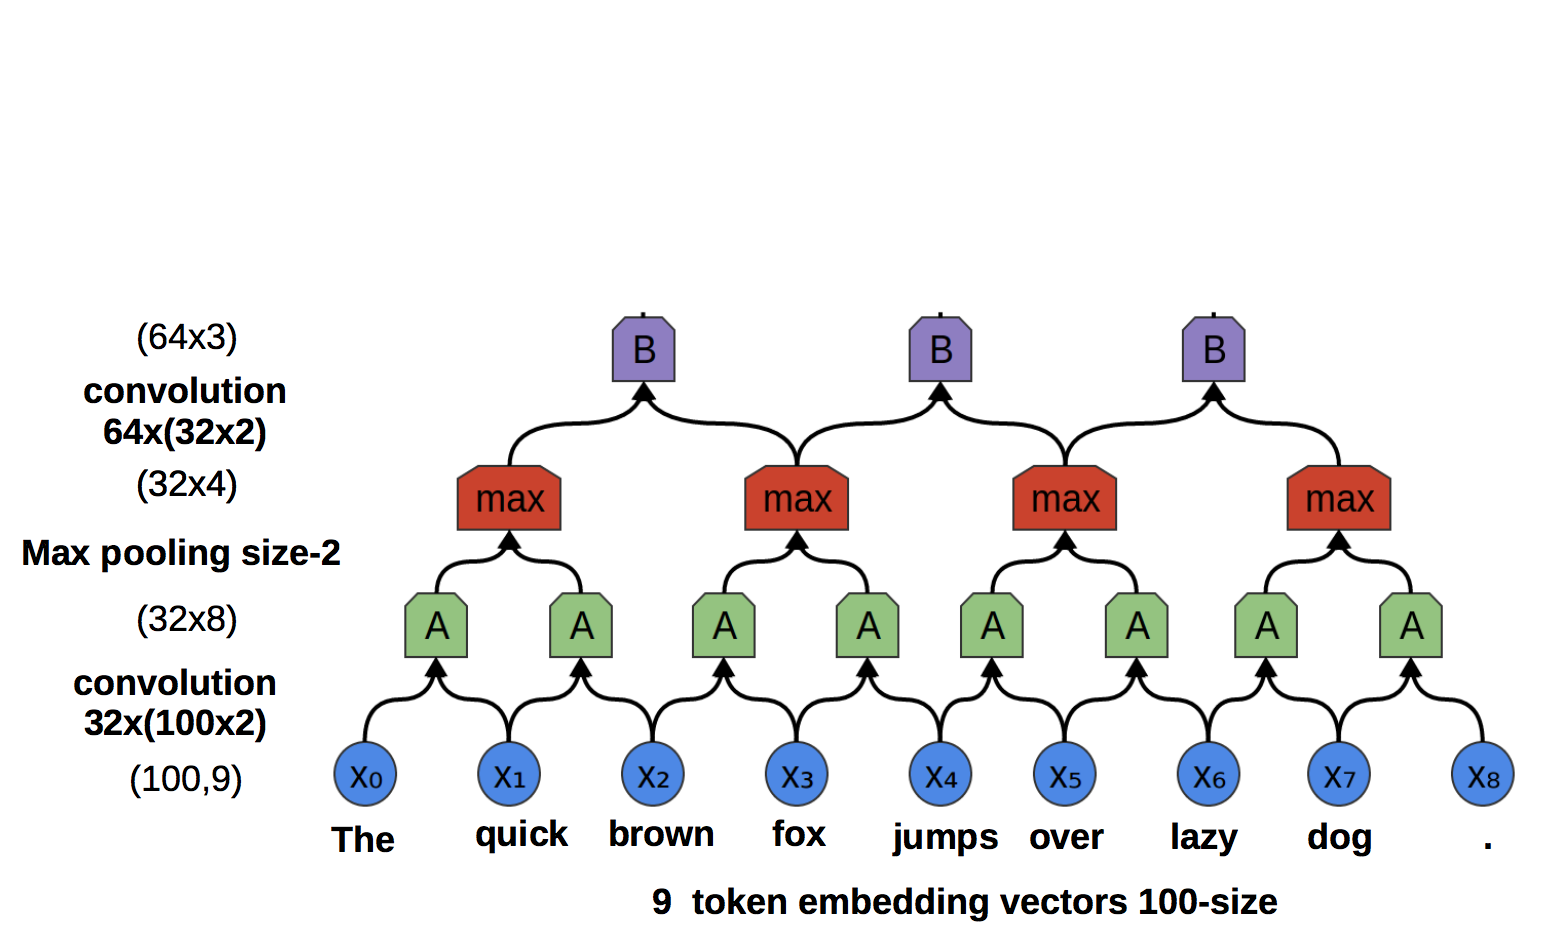
\includegraphics[width=.75\linewidth]{conv3.png}
\end{center}
\end{frame} 


\begin{frame}{Свёрточная сетка}
\begin{center}
	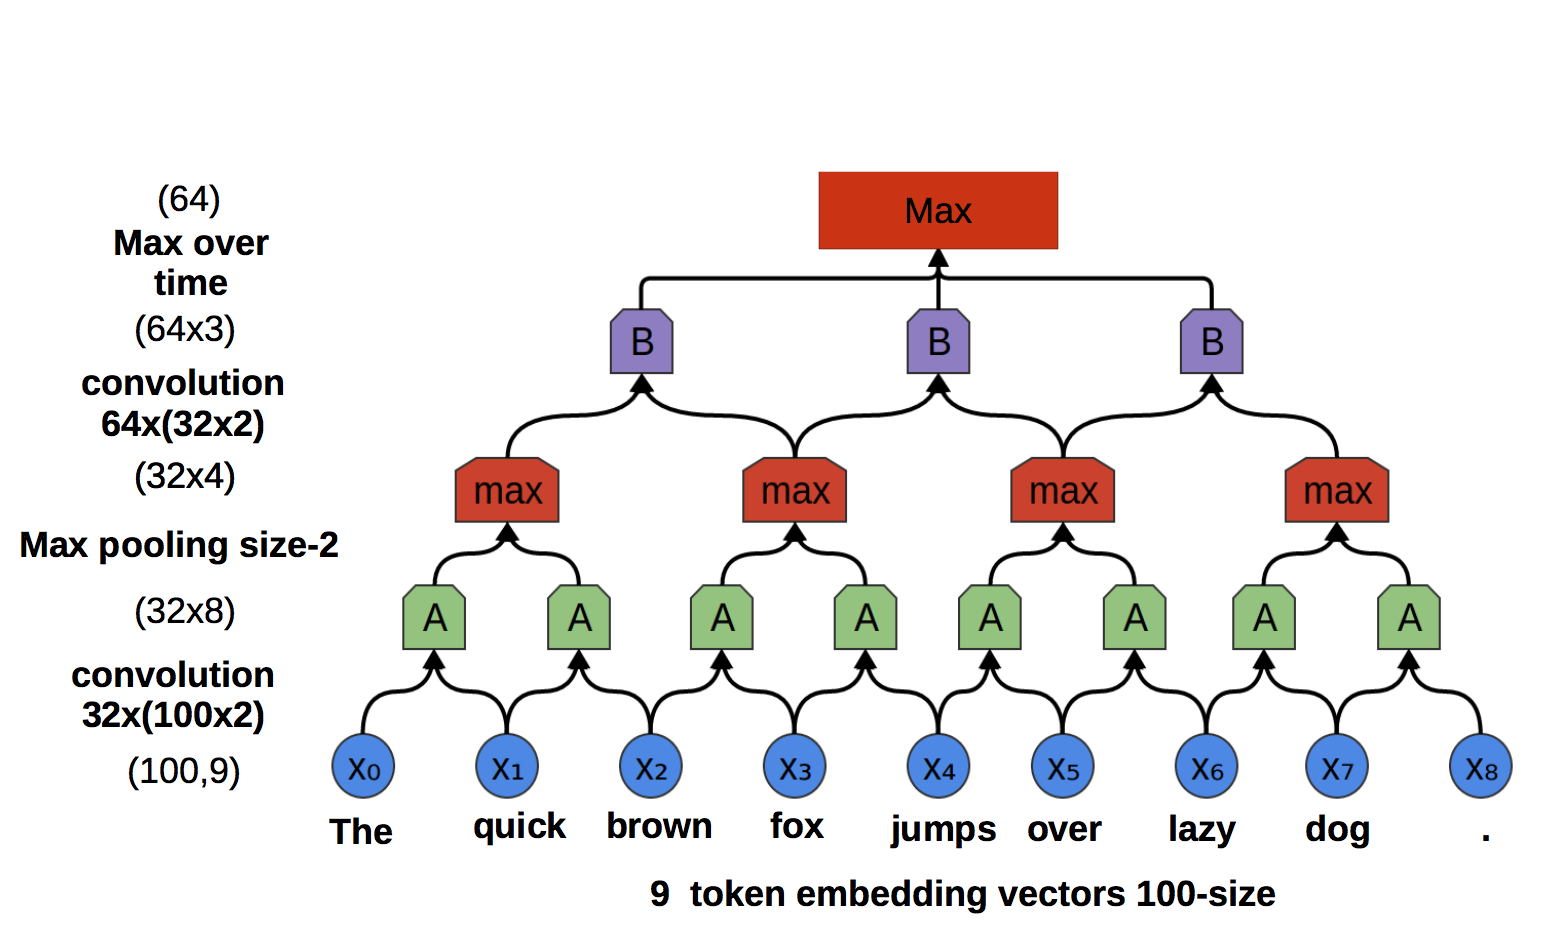
\includegraphics[width=.75\linewidth]{conv4.png}
\end{center}
\end{frame} 


\begin{frame}{Свёрточная сетка}
\begin{center}
	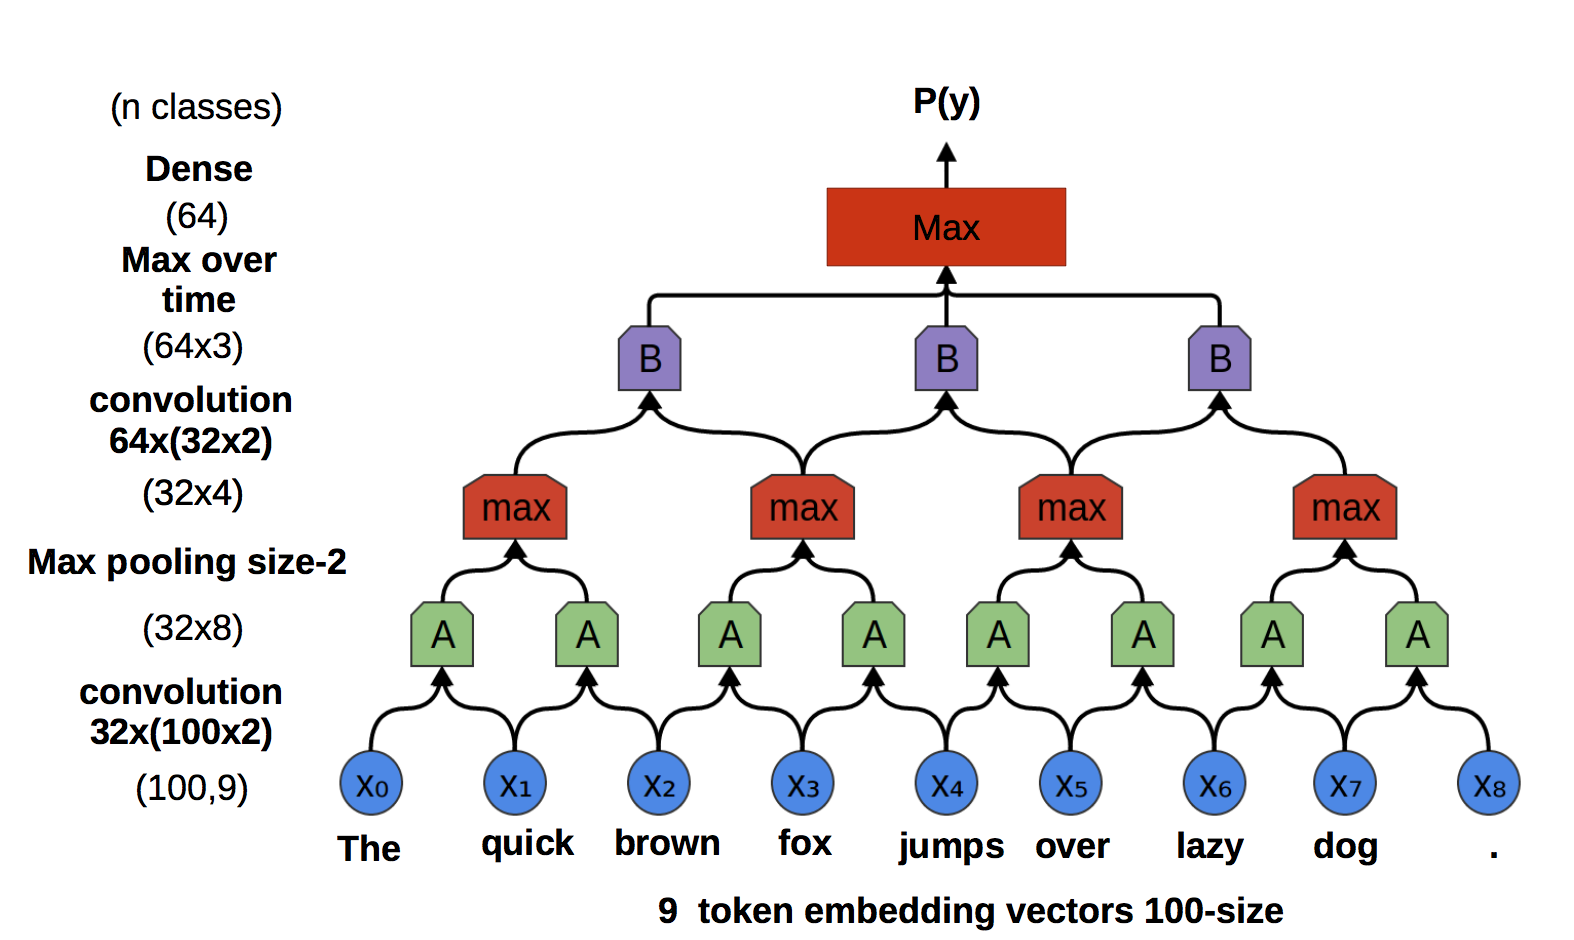
\includegraphics[width=.75\linewidth]{conv5.png}
\end{center}
\end{frame} 


\begin{frame}{Свёрточная сетка}
\begin{center}
	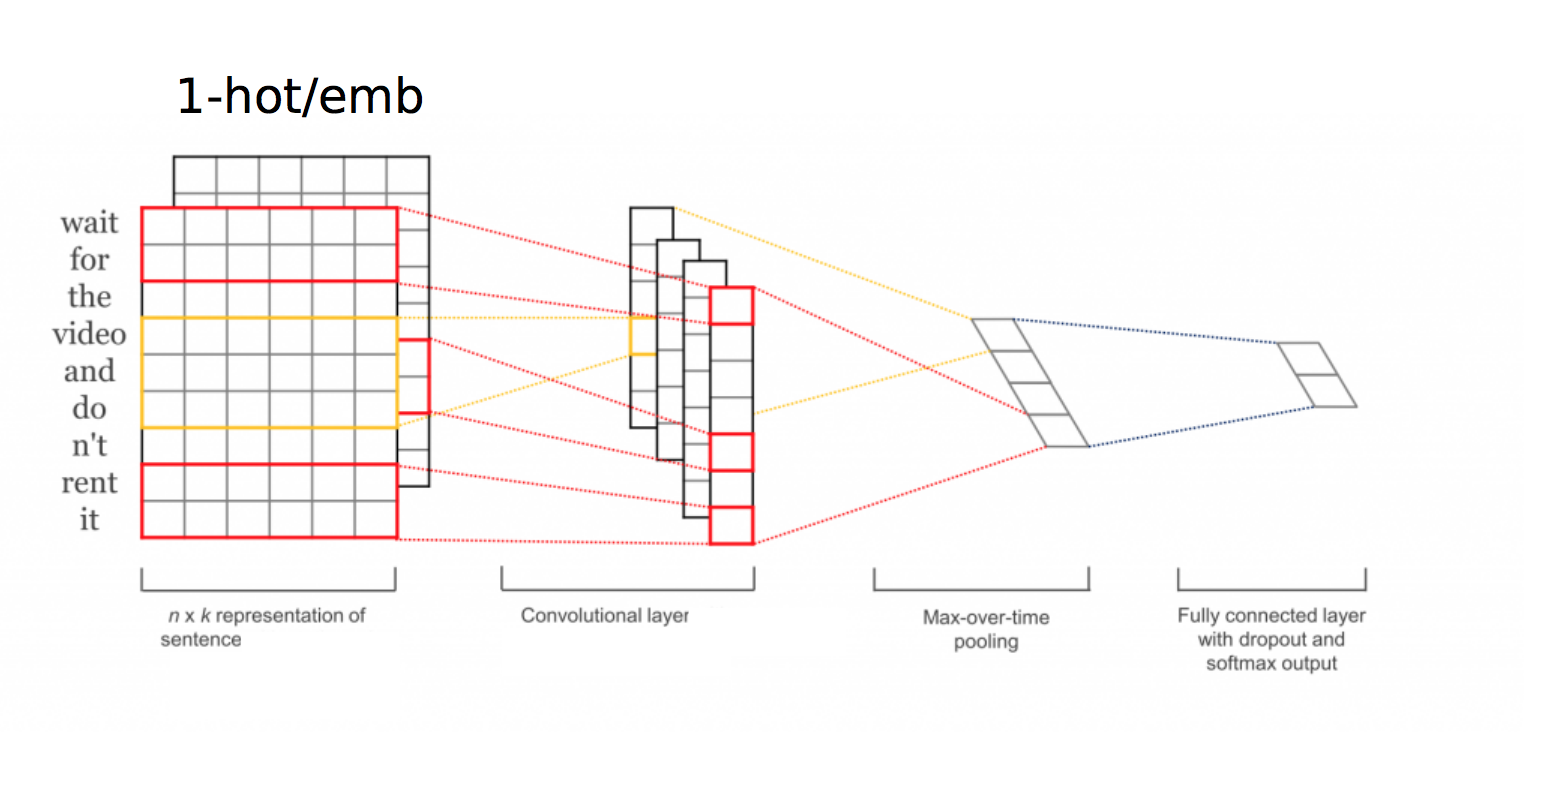
\includegraphics[width=.75\linewidth]{conv6.png}
\end{center}
\end{frame} 

% каких-нибудь картинок про новости сюда 

% сделать тут по твиттеру и сентимент-анализу кучу картинок готовых, а его дать как ДЗ 

\begin{transitionframe}
	\begin{center}
		\Huge Что такое эмбединги
	\end{center}
\end{transitionframe}

\begin{frame}{something2vec}
\begin{wideitemize} 
\item \textbf{Embedding} — это сопоставление произвольной сущности (например, узла в графе или кусочка картинки) некоторому вектору.

\item  Любую последовательность можно представить в виде эмбединга

\item  Последовательность банковских транзакций

\item  Веб-сессии (последовательность перехода по сайтам)

\item Графы взаимосвязей между пользователями 

\item Любая категориальная переменная: порядок, в котором турист посещал города; порядок, в котором юзер отранжировал сериалы и тп
\end{wideitemize} 
\end{frame} 

% Ссылка на хабровскую статью, картинки с неё 


\begin{frame}{Рекомендательные системы}
\begin{center}
	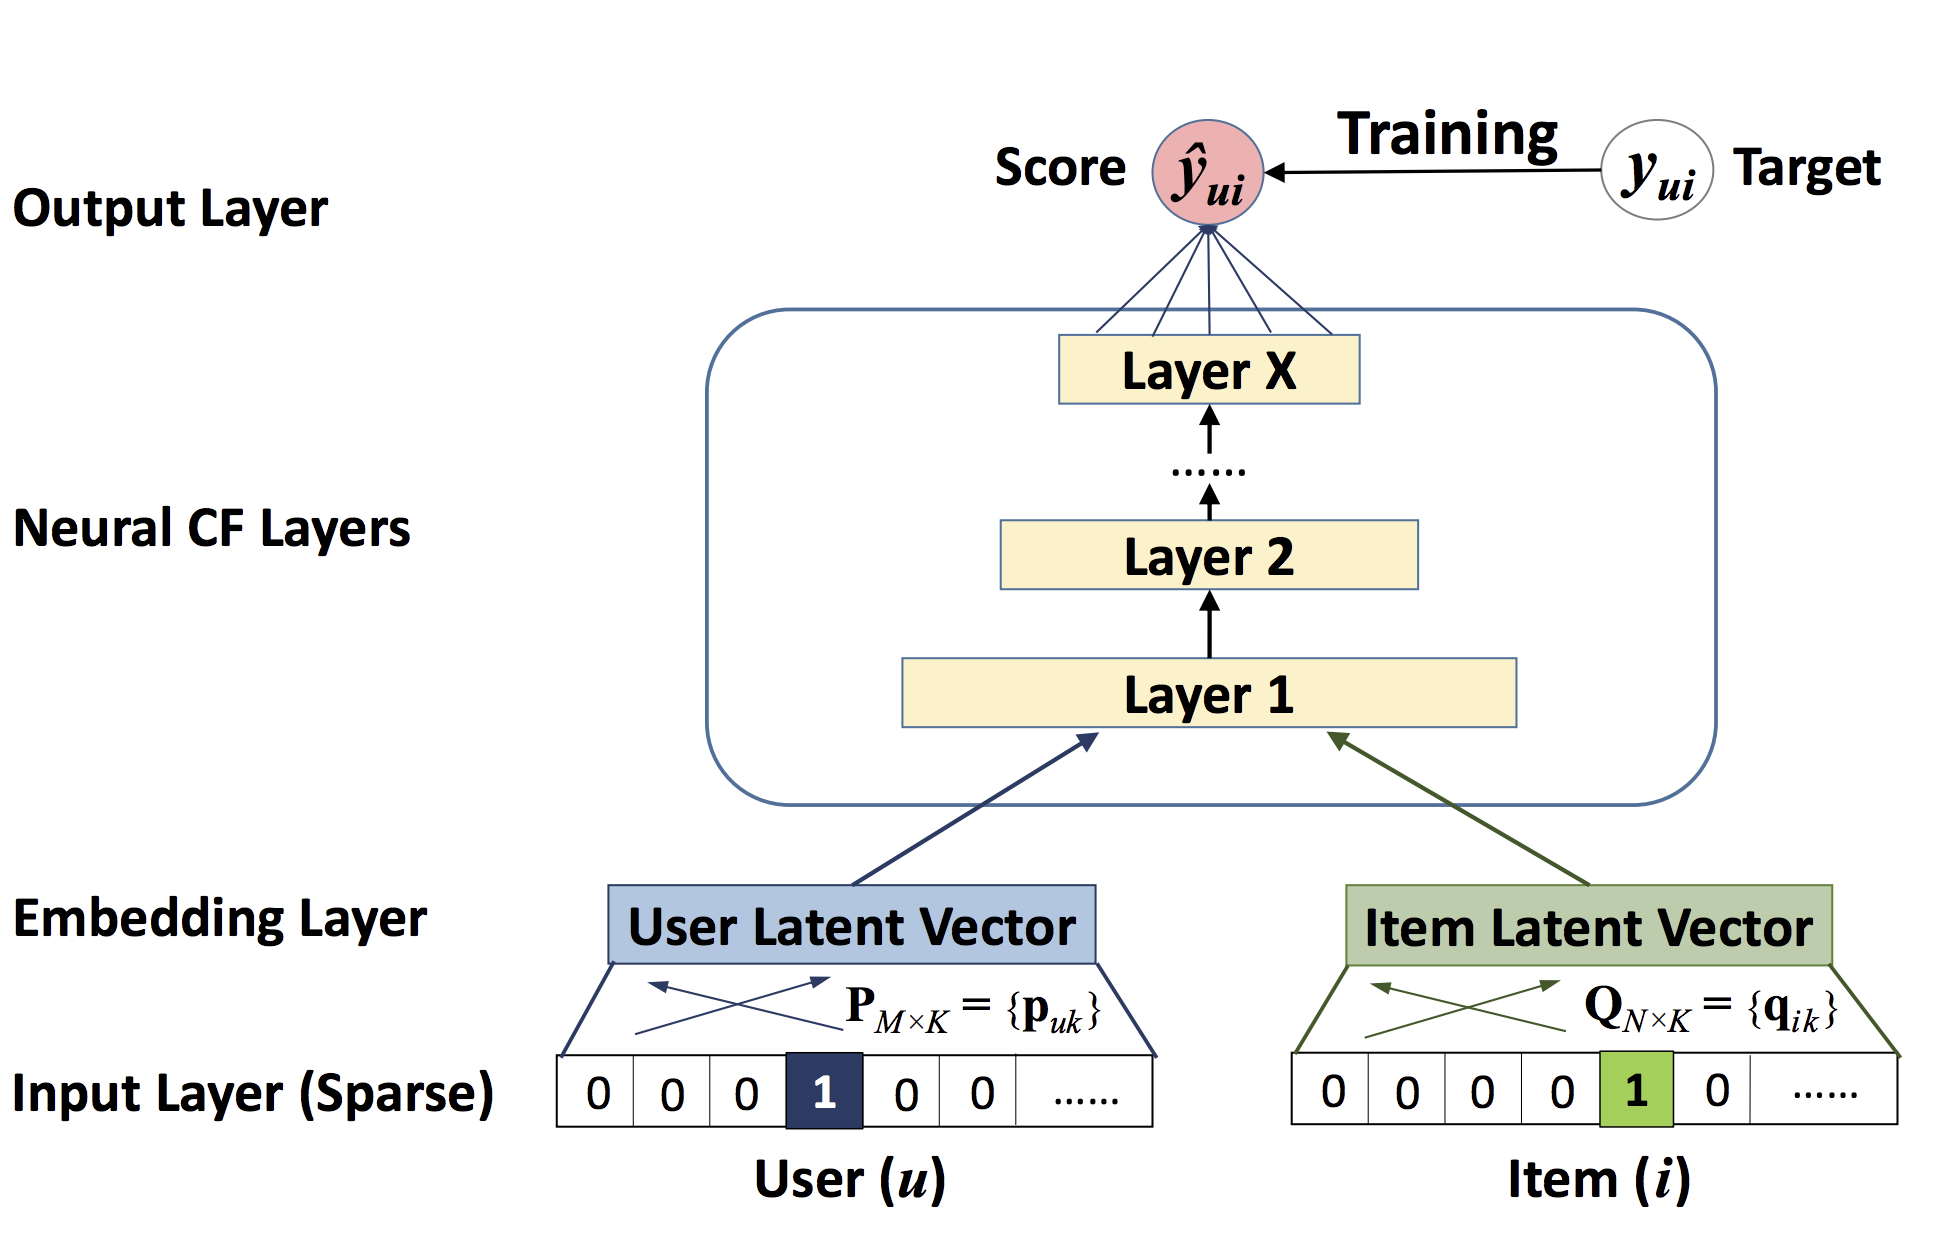
\includegraphics[width=.7\linewidth]{ncf.png}
\end{center}

\url{https://arxiv.org/pdf/1708.05031.pdf}
\end{frame}

\end{document}
